% Trust Without Receipts -- IEEE journal manuscript (IEEEtran, journal mode).
% Compiles with pdfLaTeX (Overleaf default) or XeLaTeX/Tectonic.
% Every number in Section VI is produced by backend/evals/paper/*.py; see
% backend/evals/paper/README.md for the command that regenerates each one.
\documentclass[journal]{IEEEtran}

\usepackage[T1]{fontenc}
\usepackage{cite}
\usepackage{amsmath,amssymb}
\usepackage{graphicx}
\usepackage{booktabs}
\usepackage{array}
\usepackage{multirow}
\usepackage{url}
\usepackage{tikz}
\usetikzlibrary{arrows.meta,positioning,calc,patterns}
\usepackage[hidelinks]{hyperref}

\newcommand{\Rs}{Rs.\,}
\newcommand{\code}[1]{\texttt{#1}}
\hyphenation{Errandly Post-gre-SQL}

\begin{document}

\title{Trust Without Receipts: Collusion-Aware Social Dispatch and Price-Claim Assessment for Campus Errand Platforms}

\author{Chris~Martin~Mattam,
        Ujjwal~Gogoi,
        Sanskriti~Sajlal,
        and~Ranjithkumar~S%
\thanks{The authors are with the School of Computer Science and Engineering,
Vellore Institute of Technology, Vellore 632014, Tamil Nadu, India.}%
}

\markboth{Manuscript submitted for review}%
{Mattam \MakeLowercase{\textit{et al.}}: Trust Without Receipts}

\maketitle

\begin{abstract}
Delivery platforms check a courier's expenses against a menu, a catalogue or a
receipt. A campus errand platform has none of these: when a student runner buys a
Rs.~20 puff at a hostel canteen, the claim is the only record of the price. We
present Errandly, a peer-to-peer campus errand platform, and a problem its design
creates: the dispatcher prefers friends, so money circulating inside honest friend
groups resembles collusion. We flag only money cycles among mutual
friends, then test each flagged group against an acceptance model fitted to logged
dispatch rounds from outside every suspected group. Price claims are bound to the
lines the requester ordered and judged against a one-vote-per-runner reference held
inside an administrator's band. In simulated semesters on a 1,200-student campus
that run the production code, with 30 seeds per setting, the cycle search alone
reached an F1 score of 0.96. Structure-only and money-only baselines found almost no
ring member, and two graph-mining baselines reached at most 0.48. The end-to-end pipeline, cycle search plus policy test,
reached 0.93 to 0.97 when rings were careless and 0.87 to 0.88 when they were
coordinated. The first version of the test, which reused the router's own scores,
incorrectly suppressed 146 of 149 coordinated-ring flags. The price reference stayed
at the true price with 60\% dishonest runners. We also identify a limit no such test
can pass: honest favour-trading and careful collusion leave the same logs. All
results come from simulation.
\end{abstract}

\begin{IEEEkeywords}
Collusion, fraud detection, peer-to-peer computing, reputation systems, social
networks, trust management.
\end{IEEEkeywords}

%======================================================================
\section{Introduction}
%======================================================================

\IEEEPARstart{O}{n} a residential campus, students already run errands for each
other. Someone walking past the canteen brings dinner back to a friend in the
hostel; someone going to the main gate collects a parcel for a roommate. Errandly
turns this habit into a platform. A student posts an errand with a drop point and
a fee, a nearby verified student accepts it, and the requester's money sits in
escrow until the handoff is confirmed. The system is a working prototype with an
Android and iOS client, a web client and an event-driven backend. It has not yet
been piloted with students, so every result in this paper comes from tests and
simulations of the code as built.

The hard part is not matching. Commercial delivery platforms control expense fraud
by knowing what things cost. Restaurant menus are integrated, and grocery orders are
checked against a catalogue or a scanned receipt \cite{alnaggar2021crowdsourced,le2019supply}.
A campus canteen offers none of that. It has no point-of-sale integration, no
published price list and no receipt for a loose samosa. The runner pays at the
counter and types in what it cost, and that number is the only record of the
transaction. Neither the requester nor the platform can check it.

This one property spreads through the whole system. Reimbursement can no longer be
verified, only judged for plausibility. Plausibility needs a reference price, which
has to be estimated from earlier claims made by the same people the reference will
police. An estimator that learns from those claims can be steered by them, which is
the situation studied as performative prediction \cite{perdomo2020performative}.
Judgement then falls on people rather than documents, so reputation carries real
weight, and because reputation decides who is offered work, repairing a damaged
reputation pays. Repair is easiest among friends. The friendship graph that lets the
platform prefer trusted runners is therefore the same structure that makes
collusion cheap. Coleman described network closure as the source of the trust and
sanctions that hold a group together \cite{coleman1988social}. On an errand
platform, the same closure lets a group coordinate against everyone outside it.

There is a second, quieter problem. Errandly offers each errand to the requester's
friends before strangers. Honest friends therefore end up running each other's
errands more often than chance would predict, and their money circulates inside
the group. A detector that reads in-group circulation as evidence of collusion is
then partly reading the router's own output. This is the shape of the runaway
feedback loops described for predictive policing \cite{ensign2018runaway} and of
algorithmic confounding in recommender systems \cite{chaney2018algorithmic}: the
system's decisions produce the data that later judges the people affected by them.

This paper is about that interaction between dispatch and detection, and about the
price-claim checks that make the platform usable at all. Our contributions are as
follows.

\begin{enumerate}
\item We formulate \emph{catalogue-free} errand commerce, in which expenditure is
unverifiable by construction, and give a threat model in which a successful attack
needs no forged record at all (Section~\ref{sec:model}).
\item We show that a social dispatcher and a collusion detector that share one
friendship graph interfere, and we measure by how much: staging offers by friendship
distance doubles the share of an honest group's errands that stay inside the group,
and a cycle detector that ignores this flags honest friend groups
(Sections~\ref{sec:eval-rings} and~\ref{sec:eval-dispatch}).
\item We introduce \emph{policy-conditioned evidence}. Every dispatch round is
logged, a small share of rounds is offered without the social boost, an acceptance
model is fitted to logged acceptances by people outside every suspected group, and a
group's in-group takes are compared with what that model predicts through a
Poisson-binomial $z$ statistic. We report where this clears honest groups, why the
first version, which reused the router's own scores, cleared coordinated rings, and
the limit no such test can pass: deliberate in-group routing by honest friends and
by a careful ring leave the same logs (Sections~\ref{sec:design-policy}
and~\ref{sec:eval-policy}).
\item We separate structure from evidence in collusion detection. Neighbourhood
closure discounts trust but never accuses anyone; an accusation needs a cycle of
qualified payment legs among mutual friends. We compare it with single-signal
baselines and with two standard graph-mining baselines, densest-block peeling and
label-propagation communities (Section~\ref{sec:eval-rings}).
\item We describe price-claim assessment against a reference estimated with one vote
per runner inside an administrator's band, with runners who habitually claim just
under the limit denied a vote, claims bound to the lines the requester ordered, and
shop-level partial pooling. We measure money lost and time to detection under five
attacker strategies (Section~\ref{sec:eval-price}).
\end{enumerate}

The platform has not been piloted with students. Every result comes from tests and
from simulations that run the production code, and we report the failures we found,
several of which led to the code changes described in Section~\ref{sec:impl}.

Section~\ref{sec:related} positions this work against prior research.
Section~\ref{sec:model} defines the system and threat model,
Section~\ref{sec:design} presents the design and Section~\ref{sec:impl} the
implementation. Section~\ref{sec:eval} evaluates each mechanism,
Section~\ref{sec:discussion} discusses limitations, and
Section~\ref{sec:conclusion} concludes.

%======================================================================
\section{Related Work}\label{sec:related}
%======================================================================

\subsection{Crowdsourced Delivery and Spatial Task Assignment}
Alnaggar \emph{et al.} survey crowdsourced delivery platforms and classify them by
matching mechanism, target market and pay scheme \cite{alnaggar2021crowdsourced};
Le \emph{et al.} review the supply, demand and operations of crowd-shipping
\cite{le2019supply}. Spatial crowdsourcing studies how location-bound tasks should
be assigned to moving workers \cite{tong2020spatial,kazemi2012geocrowd}. These lines
of work take the task's price as given. Price anomaly detection in marketplaces,
such as the MoatPlus system of Sarpal \emph{et al.}, sets upper price bounds from
historical and proximate prices of catalogued items \cite{sarpal2023marketplace};
it assumes the catalogue we lack. Escrow services have been analysed as trusted
third parties in online auctions \cite{hu2004hope}, but an escrow can only hold an
amount that both sides agree on. In our setting the amount is the thing in dispute.

\subsection{Trust, Reputation and Sybil Resistance}
Reputation systems aggregate past feedback to predict future behaviour
\cite{resnick2000reputation,dellarocas2003digitization,josang2007survey}, and
Hoffman \emph{et al.} catalogue the attacks on them, collusion and identity
manipulation among them \cite{hoffman2009survey}. EigenTrust propagates trust
transitively through a peer network \cite{kamvar2003eigentrust}, and graph-based
trust models for social networks commonly let trust decay with path length
\cite{jiang2016trust}, which we follow. Sybil defences built on social graphs, such
as SybilGuard, rely on a sparse cut between honest and fake regions
\cite{yu2008sybilguard}, and Cheng and Friedman show that a large class of
reputation functions cannot be Sybil-proof \cite{cheng2005sybilproof}. On our
platform identity is tied to an institutional e-mail address, so fake accounts are
costly \cite{douceur2002sybil}; the attacks that remain are carried out with real
accounts. Studies of peer platforms report that ratings are shaped by reciprocity
\cite{bolton2013engineering}, inflate over time \cite{filippas2022reputation} and
respond to personal trust cues \cite{ert2016trust}. We take from these that a
rating's meaning depends on who gave it.

\subsection{Closure and Cohesion}
Coleman \cite{coleman1988social} and Granovetter \cite{granovetter1985economic}
argue that closed, embedded networks support trust and enforcement, while Burt
stresses the value of ties that bridge otherwise separate groups
\cite{burt1992structural}. The clustering coefficient of Watts and Strogatz
\cite{watts1998collective} is the usual local measure of cohesion. Community
detection methods such as modularity maximisation \cite{newman2006modularity}, the
Louvain method \cite{blondel2008fast} and label propagation \cite{raghavan2007lpa}
partition a whole graph. The closure score we use is not a new kind of measure. With
the student removed, it is a monotone transform, $c=(1-\phi)/(1+\phi)$, of the
conductance $\phi$ \cite{kannan2004clusterings} of the student's friend set, and it is
close in spirit to Burt's ego-network constraint \cite{burt1992structural}. What we need from it is narrow: a per-student
number that is cheap to refresh in plain Cypher, easy to explain to a reviewer, and
sensitive to whether a neighbourhood is sealed off from the rest of campus.
Section~\ref{sec:eval-closure} shows that the clustering coefficient does not have
the last property. The novelty is in how the score is used, as a discount on trust
that never accuses anyone, rather than in the score itself.

\subsection{Collusion and Group Fraud}
Fraud detection on review and social platforms looks for groups that act together:
fake reviewer groups \cite{mukherjee2012spotting}, spammers with abnormal rating
behaviour \cite{lim2010detecting}, accounts that act in lockstep
\cite{beutel2013copycatch} and dense blocks hidden behind camouflage edges
\cite{hooi2016fraudar}; Akoglu \emph{et al.} survey graph-based anomaly detection
\cite{akoglu2015graph}. Shilling-attack detection for recommender systems targets
injected profiles and rating time series \cite{gunes2014shilling,zhou2018shilling}.
Collusion among crowd workers has its own literature. Xu \emph{et al.} review
similarity-based, graph-based and learned detectors of worker collusion and note how
hard it is to obtain ground truth \cite{xu2025collusionreview}. Han \emph{et al.}
show that collusion can be organised anonymously at large scale and detect it with a
graph algorithm over workers' answers \cite{han2025anonymous}, and Zhang \emph{et al.}
predict fraudulent requesters on a contest platform from their centrality and
clustering in the social network \cite{zhang2026sna}. These methods share an
assumption: somewhere in the data there is a fake record, a copied answer or an
abnormal position in the network. The attack we care about breaks that assumption.
A ring's friendships are real, its errands are really run, and the ratings its
members leave each other may be perfectly sincere. More importantly for us, none of
these detectors runs beside a matcher that itself puts friends together, so none has
to separate the platform's influence from the group's.

\subsection{Truth Discovery and Robust Aggregation}
Truth discovery infers true values from conflicting sources by estimating how
reliable each source is \cite{li2016truth}; multi-truth discovery allows an object
several correct values \cite{lin2018domain}, which matches an item that costs
different amounts in different shops. Fang \emph{et al.} show that coordinated
workers can poison such aggregates \cite{fang2021poisoning}. Robust statistics gives
the tools we use: the influence curve \cite{hampel1974influence}, the median absolute
deviation and its alternatives \cite{rousseeuw1993alternatives,huber2009robust}, and
practical outlier rules based on it \cite{leys2013detecting}. Partial pooling toward
a common mean follows the empirical Bayes argument of Efron and Morris
\cite{efron1975data}.

\subsection{Feedback Loops and Logged Exploration}
Perdomo \emph{et al.} formalise predictions that change the distribution they are
evaluated on \cite{perdomo2020performative}. Ensign \emph{et al.} show how a
predictive-policing system that sends patrols where it previously found crime keeps
confirming itself \cite{ensign2018runaway}, and Chaney \emph{et al.} show how
recommender feedback homogenises behaviour \cite{chaney2018algorithmic}. Offline
evaluation of deployed systems relies on logged decision probabilities
\cite{bottou2013counterfactual} and on a small slice of randomised traffic
\cite{li2010contextual}. Our policy test borrows both ideas in a simple form: the
logged scores define a conditional-logit choice model \cite{mcfadden1974conditional},
and the number of in-group takes is a sum of independent, non-identical Bernoulli
trials \cite{wang1993number}.

\subsection{Language Models in a Fraud Pipeline}
Text sent to a language model inside an application can carry instructions aimed at
the model \cite{greshake2023not}. In our case every string the model sees is written
by the people being judged. We use a locally hosted Qwen2.5 7B model
\cite{qwen2024qwen25} and keep it advisory (Section~\ref{sec:design-llm}).

Table~\ref{tab:positioning} compares the detectors closest to ours on the three
properties that matter here.

\begin{table*}[!t]
\caption{Collusion and Fraud Detectors Closest to This Work}
\label{tab:positioning}
\centering
\footnotesize
\begin{tabular}{@{}>{\raggedright}p{0.17\textwidth}>{\raggedright}p{0.17\textwidth}>{\raggedright}p{0.26\textwidth}ccc@{}}
\toprule
Work & Setting & Evidence used & Needs a & Accounts for & Judges \\
& & & fake record & the matcher & unpriced claims \\
\midrule
Mukherjee \emph{et al.} \cite{mukherjee2012spotting} & product reviews & group
behaviour features & yes & no & no \\
CopyCatch \cite{beutel2013copycatch}, FRAUDAR \cite{hooi2016fraudar} & social and
e-commerce graphs & lockstep edges, dense blocks & yes & no & no \\
Han \emph{et al.} \cite{han2025anonymous}; review \cite{xu2025collusionreview} &
crowdsourced labelling & answer similarity, worker graphs & yes & no & no \\
Zhang \emph{et al.} \cite{zhang2026sna} & contest crowdsourcing & centrality and
clustering of requesters & no & no & no \\
Fang \emph{et al.} \cite{fang2021poisoning} & truth discovery & source reliability &
yes & no & no \\
MoatPlus \cite{sarpal2023marketplace} & online marketplace & catalogue price history
& no & no & catalogued only \\
Ensign \emph{et al.} \cite{ensign2018runaway} & predictive policing & (analysis of a
feedback loop) & no & yes & no \\
\textbf{This work} & campus errands & money cycles among friends, tested against a
fitted model of logged routing & no & yes & yes \\
\bottomrule
\end{tabular}
\end{table*}

%======================================================================
\section{System and Threat Model}\label{sec:model}
%======================================================================

\subsection{Actors and Errand Lifecycle}
Students register with an institutional e-mail address verified by a one-time
code. Any student can post an errand as a \emph{requester} or accept one as a
\emph{runner}; administrators maintain reference prices and review flags. An errand
has a drop point, a fee, an optional amount of cash to collect (for example at the
gate) and an item list. Items are of three kinds: menu items from vendors registered
on the platform, packaged goods with a printed maximum retail price (MRP), and
\emph{loose-priced} items such as canteen food that carry no printed price. Only the
last kind is reimbursed on the runner's word.

Fig.~\ref{fig:lifecycle} shows the lifecycle. Money is placed in escrow before any
runner sees the errand. Offers go out in timed tiers (Section~\ref{sec:design-dispatch}).
Acceptance takes a Redis lock and then a row lock, so exactly one runner wins a
race. Before marking the errand picked up, the runner must report the price of
every loose-priced line, and each line is judged at that moment. Settlement happens
once, when the requester confirms completion.

\begin{figure}[!t]
\centering
% Errand lifecycle, with where money is held and where evidence is produced.
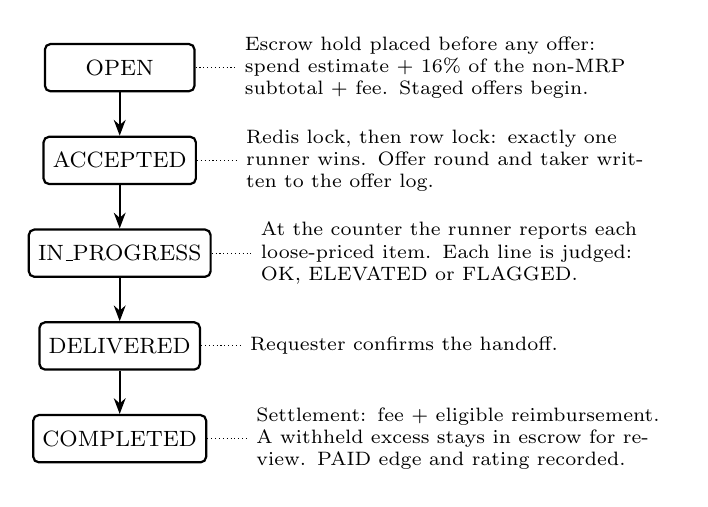
\begin{tikzpicture}[
  font=\footnotesize,
  st/.style={draw, thick, rounded corners=2pt, minimum width=19mm, minimum height=6mm, align=center},
  note/.style={align=left, font=\scriptsize, text width=52mm, anchor=west},
  flow/.style={-{Stealth[length=2mm]}, thick},
  link/.style={densely dotted},
  node distance=5.5mm]
  \node[st] (open) {OPEN};
  \node[st, below=of open] (acc) {ACCEPTED};
  \node[st, below=of acc] (prog) {IN\_PROGRESS};
  \node[st, below=of prog] (del) {DELIVERED};
  \node[st, below=of del] (done) {COMPLETED};
  \foreach \a/\b in {open/acc, acc/prog, prog/del, del/done} \draw[flow] (\a) -- (\b);

  \node[note, right=5mm of open] (n1) {Escrow hold placed before any offer: spend
    estimate + 16\% of the non-MRP subtotal + fee. Staged offers begin.};
  \node[note, right=5mm of acc] (n2) {Redis lock, then row lock: exactly one runner wins.
    Offer round and taker written to the offer log.};
  \node[note, right=5mm of prog] (n3) {At the counter the runner reports each loose-priced
    item. Each line is judged: OK, ELEVATED or FLAGGED.};
  \node[note, right=5mm of del] (n4) {Requester confirms the handoff.};
  \node[note, right=5mm of done] (n5) {Settlement: fee + eligible reimbursement. A
    withheld excess stays in escrow for review. PAID edge and rating recorded.};
  \foreach \s/\n in {open/n1, acc/n2, prog/n3, del/n4, done/n5} \draw[link] (\s.east) -- (\n.west);
\end{tikzpicture}

\caption{Errand lifecycle. Money is held before any offer goes out, every
loose-priced line is judged at the counter, and settlement pays only the eligible
amount.}
\label{fig:lifecycle}
\end{figure}

\subsection{Graphs, Logs and Claims}\label{sec:defs}
Let $U$ be the students on one campus. The \emph{friendship graph}
$G_F=(U,E_F)$ is undirected; an edge exists only for an accepted friend request and
records when it was accepted. We write $N(u)$ for the friends of $u$.

The \emph{payment graph} $G_P$ is a directed multigraph. A completed errand $e$
posted by $a$ and run by $b$ adds an edge $a\to b$ with time $t_e$ and amount
$x_e$, the fee plus any cash the runner collected for $a$. The reimbursement for
goods is deliberately left out. It repays a shop for things $a$ received, so it is
not value transferred from $a$ to $b$, and counting it would make a large grocery run
for a friend look like a large gift.

The \emph{offer log} records, for every dispatch round, the requester, each
candidate's distance, friendship distance, trust, reputation, penalty and resulting
score, whether the round was exploratory, and who accepted.

An errand's \emph{order lines} are what the requester asked for: a name, a quantity
and, for an item picked from the administrator's price list, a link to its
reference. A \emph{claim} is the runner's report of the unit price paid for one order
line. The unit is one of whatever the line names (one puff, one bottle), and the
claimed quantity may not exceed the quantity ordered. A claim records the runner,
item, shop, unit price, quantity, the reference and allowance it was judged against,
and the verdict.

\emph{Reference notation.} For item $k$, $r_k$ is the campus reference in force.
The administrator sets its initial value and a band $[L_k,U_k]$;
$\hat r_k$ is the estimate computed from recent claims, which replaces $r_k$ only
inside the band (Section~\ref{sec:design-reference}); and $r^*_{k,s}$ is the
shop-adjusted value used to judge a claim made at shop $s$ (equation~\eqref{eq:store}).
Where the shop is unknown or barely observed, $r^*_{k,s}=r_k$.

\emph{Outcome terms.} We use five words with fixed meanings. A claim, a runner or a
group is \emph{flagged} when a rule writes a flag record; a flag is evidence, not a
verdict. A ring flag is \emph{suppressed} when the policy test
(Section~\ref{sec:design-policy}) finds the group's in-group activity explained, in
which case no flag is written. A flag is \emph{reviewed} when an administrator marks
it upheld or dismissed. A student is \emph{sanctioned} when an action is applied to
their account: a warning, a rank penalty, a pause on running or a suspension. A
student is \emph{cleared} when a dismissal releases withheld money and lifts any pause
that the remaining flags no longer justify (Section~\ref{sec:design-claims}).

\subsection{Threat Model}
The attacker is a verified student who wants to be paid more than the work is worth,
acting alone or with genuine friends. We assume the attacker knows every rule in this
paper, can coordinate with friends over chat, and can run real errands at real cost.
We assume the attacker cannot create accounts in bulk, because each needs an
institutional address, and cannot tamper with the server or its logs.

Fig.~\ref{fig:threat} and Table~\ref{tab:threat} show the campaign we design
against. The loop closes because reputation decides who is offered work: a runner
whose rank has fallen needs to repair it before reaching new victims, so repairing it
is a precondition of the fraud rather than vanity. Stages 4 and 5 need no forged data.
The friends are real, the errands are run, and the five-star ratings may be sincere.

Out of scope are a shopkeeper who quotes a false price on the runner's behalf,
shared accounts, coercion, a compromised administrator and spoofed device locations.

\begin{figure}[!t]
\centering
% The attacker's loop. Reputation gates access to work, so repairing it is
% a precondition for reaching new victims, not vanity.
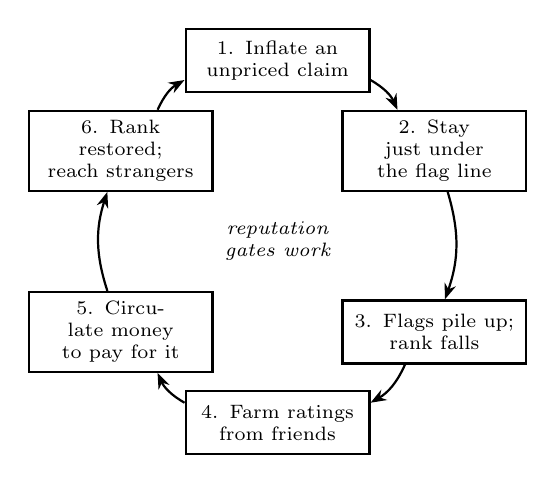
\begin{tikzpicture}[
  font=\scriptsize,
  stage/.style={draw, thick, rectangle, align=center, text width=21mm, minimum height=8mm},
  flow/.style={-{Stealth[length=2mm]}, thick}]
  \def\R{23mm}
  \foreach \i/\t in {
      1/{1. Inflate an\\unpriced claim},
      2/{2. Stay just under\\the flag line},
      3/{3. Flags pile up;\\rank falls},
      4/{4. Farm ratings\\from friends},
      5/{5. Circulate money\\to pay for it},
      6/{6. Rank restored;\\reach strangers}} {
    \node[stage] (s\i) at ({90 - (\i-1)*60}:\R) {\t};
  }
  \foreach \i/\j in {1/2, 2/3, 3/4, 4/5, 5/6, 6/1}
    \draw[flow] (s\i) to[bend left=18] (s\j);
  \node[align=center, font=\scriptsize\itshape] at (0,0) {reputation\\gates work};
\end{tikzpicture}

\caption{The attacker's loop. Each stage is answered by a control in
Table~\ref{tab:threat}.}
\label{fig:threat}
\end{figure}

\begin{table}[!t]
\caption{Attack Stages and the Controls That Answer Them}
\label{tab:threat}
\centering
\footnotesize
\begin{tabular}{@{}c>{\raggedright}p{0.36\columnwidth}>{\raggedright\arraybackslash}p{0.47\columnwidth}@{}}
\toprule
Stage & Attacker move & Control (Section) \\
\midrule
1 & inflate the price of a loose item & reference with band; withhold excess
(\ref{sec:design-claims}, \ref{sec:design-reference}) \\
2 & keep every claim just under the limit & distribution rule; no vote on the
reference (\ref{sec:design-claims}) \\
3 & absorb flags; rank falls & strike ladder; capped rank penalty
(\ref{sec:design-claims}, \ref{sec:design-dispatch}) \\
4 & farm ratings from friends & one vote per rater; concentration discount
(\ref{sec:design-reputation}) \\
5 & circulate money to fund stage 4 & cycles among friends; policy test
(\ref{sec:design-rings}, \ref{sec:design-policy}) \\
6 & make farmed errands look real & language channel, advisory only
(\ref{sec:design-llm}) \\
\bottomrule
\end{tabular}
\end{table}

%======================================================================
\section{Design}\label{sec:design}
%======================================================================

\subsection{Overview}
Fig.~\ref{fig:arch} shows the architecture. PostgreSQL is the only source of truth.
Every state change writes a domain event to an outbox table in the same transaction,
a relay publishes it to Kafka, and four consumer groups handle notifications,
analytics, settlement and the projection of friendships and payments into Neo4j. The
graph is a derived read model: nothing on a request path writes to it, it can be
rebuilt from the event log, and every read from it sits behind a circuit breaker. A
scheduler escalates offers, refreshes graph metrics and runs the fraud sweeps.
Table~\ref{tab:params} collects the parameters introduced in the rest of this section.

\begin{figure*}[!t]
\centering
% System architecture in two lanes. Upper lane: the synchronous request path.
% Lower lane: asynchronous event traffic and background jobs. Solid arrows are
% calls made inside a request; dashed arrows are events or read-model traffic.
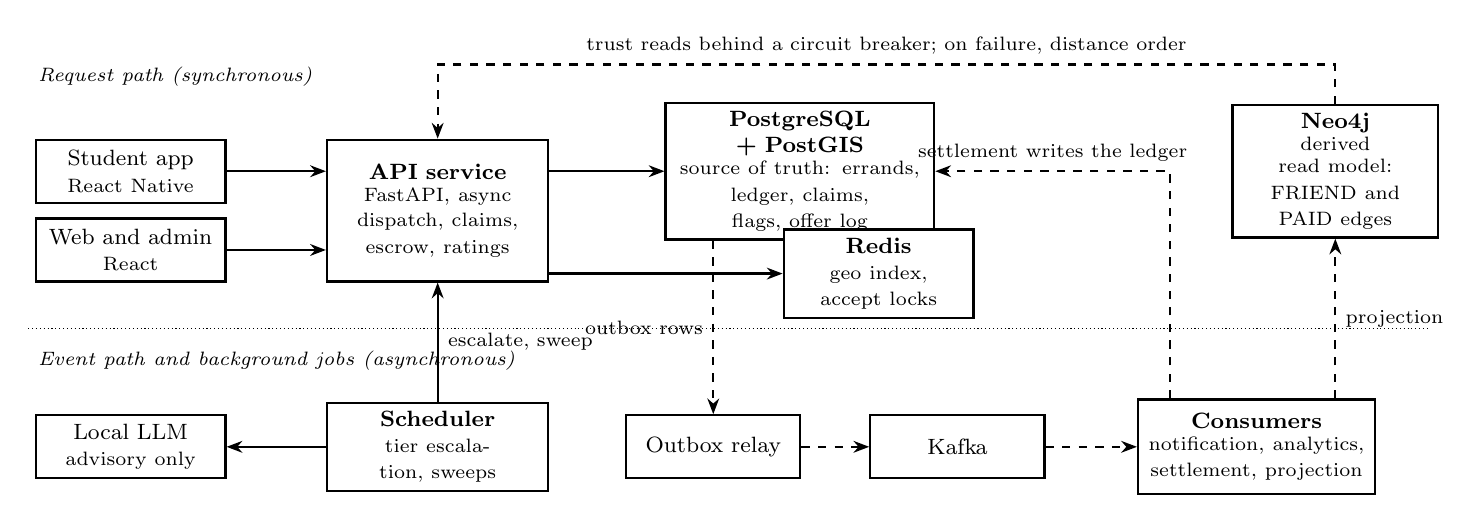
\begin{tikzpicture}[
  font=\footnotesize,
  box/.style={draw, thick, rectangle, align=center, inner sep=3pt, minimum height=8mm,
              text width=#1, fill=white},
  box/.default=24mm,
  sync/.style={-{Stealth[length=2mm]}, thick},
  async/.style={-{Stealth[length=2mm]}, thick, dashed},
  lane/.style={font=\scriptsize\itshape, anchor=west}]

  % lane labels and separator
  \node[lane] at (-2mm, 21mm) {Request path (synchronous)};
  \node[lane] at (-2mm, -15mm) {Event path and background jobs (asynchronous)};
  \draw[densely dotted] (-2mm, -11mm) -- (176mm, -11mm);

  % ---- upper lane
  \node[box=22mm] (mob) at (11mm, 9mm) {Student app\\\scriptsize React Native};
  \node[box=22mm] (web) at (11mm, -1mm) {Web and admin\\\scriptsize React};
  \node[box=26mm, minimum height=18mm] (api) at (50mm, 4mm)
       {\textbf{API service}\\\scriptsize FastAPI, async\\[1pt]\scriptsize dispatch, claims,\\
        \scriptsize escrow, ratings};
  \node[box=32mm, minimum height=12mm] (pg) at (96mm, 9mm)
       {\textbf{PostgreSQL + PostGIS}\\\scriptsize source of truth: errands,\\
        \scriptsize ledger, claims, flags, offer log};
  \node[box=22mm] (rd) at (106mm, -4mm) {\textbf{Redis}\\\scriptsize geo index, accept locks};
  \node[box=24mm, minimum height=12mm] (neo) at (164mm, 9mm)
       {\textbf{Neo4j}\\\scriptsize derived read model:\\\scriptsize FRIEND and PAID edges};

  % ---- lower lane
  \node[box=22mm] (llm) at (11mm, -26mm) {Local LLM\\\scriptsize advisory only};
  \node[box=26mm] (sch) at (50mm, -26mm) {\textbf{Scheduler}\\\scriptsize tier escalation, sweeps};
  \node[box=20mm] (relay) at (85mm, -26mm) {Outbox relay};
  \node[box=20mm] (kafka) at (116mm, -26mm) {Kafka};
  \node[box=28mm, minimum height=12mm] (cons) at (154mm, -26mm)
       {\textbf{Consumers}\\\scriptsize notification, analytics,\\\scriptsize settlement, projection};

  % ---- request path
  \draw[sync] (mob.east) -- (api.west |- mob.east);
  \draw[sync] (web.east) -- (api.west |- web.east);
  \draw[sync] (api.east |- pg.west) -- (pg.west);
  \draw[sync] (api.east |- rd.west) -- (rd.west);
  \draw[async] (neo.north) -- ++(0, 5mm) -| node[pos=0.25, above, font=\scriptsize]
       {trust reads behind a circuit breaker; on failure, distance order} (api.north);

  % ---- event path
  \draw[async] ([xshift=-11mm]pg.south) -- node[left, font=\scriptsize] {outbox rows}
       ([xshift=-11mm]pg.south |- relay.north);
  \draw[async] (relay) -- (kafka);
  \draw[async] (kafka) -- (cons);
  \draw[async] (neo.south |- cons.north) -- node[right, font=\scriptsize] {projection} (neo.south);
  \draw[async] ([xshift=-11mm]cons.north) |- node[pos=0.75, above, font=\scriptsize]
       {settlement writes the ledger} (pg.east);
  \draw[sync] (sch.north) -- node[right, font=\scriptsize] {escalate, sweep} (sch.north |- api.south);
  \draw[sync] (sch.west) -- (llm.east);
\end{tikzpicture}

\caption{Architecture in two lanes. The upper lane is the request path, the lower
lane the event path and background jobs. Solid arrows are synchronous calls; dashed
arrows are events or read-model traffic. Losing Neo4j degrades matching to distance
order and never blocks a request.}
\label{fig:arch}
\end{figure*}

\subsection{Assessing a Price Claim}\label{sec:design-claims}
A claim must first be tied to the right reference, because a claim that matches no
reference is never checked at all. On an itemised order the claim is bound to one of
the order's own lines. Its name is matched against the names of those lines, exactly
after normalisation and otherwise by fuzzy matching. A line the requester picked from
the administrator's price list is then judged against that line's reference, whatever
the runner calls it. A name that matches no line is refused, and so is a quantity
above the quantity ordered. Before this rule, a runner could rename a priced item
(``zzq special'') until it matched nothing and be paid unchecked; Section~\ref{sec:eval-price}
measures the difference. On an errand with no itemised lines the claimed name is
mapped to a campus-wide key instead. Deterministic rules handle case, punctuation,
plurals and common abbreviations (``chkn puf'' becomes ``chicken puff''), and fuzzy
matching with a similarity threshold of 0.86 handles typos against the keys a campus
already prices. A language model may \emph{suggest} aliases for names that recur
unmatched, but nothing is judged against an alias until an administrator approves
it.

For item $k$ with reference price $r_k$, the allowance is
\begin{equation}
\tau_k = \min\bigl(\max(0.40\,r_k,\ \Rs 5),\ \Rs 20\bigr), \label{eq:tolerance}
\end{equation}
where the percentage, floor and cap are per-item settings. A flat allowance would
be 80\% of a Rs.~25 puff and 4\% of a Rs.~500 grocery run; scaling it protects the
cheap items that make up most of the traffic. A claimed unit price $c$ at shop $s$,
judged against $r^*_{k,s}$ (Section~\ref{sec:design-reference}), is
\emph{FLAGGED} if $c-r^*_{k,s}>\tau_k$, \emph{ELEVATED} if $0<c-r^*_{k,s}\le\tau_k$
and \emph{OK} otherwise. For a line of quantity $q$, a flagged claim is reimbursed at
$q\,r^*_{k,s}$ and the excess stays in escrow for review; the other two are paid
$q\,c$ in full. An item with no reference (the cold-start
case, Section~\ref{sec:design-reference}) is paid as claimed, up to the escrow hold,
and becomes evidence for one.

One high claim is not fraud; prices do rise. Sanctions therefore key on a pattern,
and only price-claim flags count toward it; ring and rating-farming flags never feed
the ladder, because they are relational inferences that a person has to weigh. With
3, 5 and 8 flagged errands within 30 days the system applies, automatically, a
warning, a 0.5-star reputation penalty and a seven-day pause on running. These three
steps are temporary and reversible. The fourth, account suspension, needs 12 flags
that an administrator has \emph{upheld}; open flags alone stop at the pause. Flags
are counted per errand, so one receipt with four inflated lines is one incident.
Every sanction notifies the student with the reason and a route to an administrator.
That is the appeal path. When an administrator dismisses a flag, the withheld money
is paid to the runner, the claim is restored as evidence, and a running pause that
the remaining flags no longer justify is lifted. The strike stays on record, marked
as lifted.

A runner can also sit just under the limit on every claim. A claim is \emph{near the
line} if $c-r^*_{k,s}\ge0.6\,\tau_k$. A runner with at least four near-line claims in 30
days, forming at least 60\% of their judged claims, receives a
\code{PERSISTENT\_NEAR\_THRESHOLD} flag. Requiring a share as well as a count keeps
a busy honest runner, whose elevated claims are diluted by ordinary ones, out of it.
No money is withheld for this flag, because no single claim broke a rule.

\subsection{Estimating References From Adversarial Claims}\label{sec:design-reference}
The administrator sets, for each loose-priced item, a reference and a band
$[L_k,U_k]$. An hourly job re-estimates the reference from the last 30 days of
claims. Flagged claims are excluded, and so are all claims by runners under an open
or upheld near-line flag. Their claims are individually legal, which is why they
would otherwise drag the line upward. Claims are grouped by runner and each
runner contributes one vote, the median of their own claims $m_i$. With
$M=\operatorname{med}_i m_i$ and $\mathrm{MAD}=\operatorname{med}_i|m_i-M|$, votes with
$|m_i-M|>3\times1.4826\times\mathrm{MAD}$ are dropped and the estimate is the median of
the rest \cite{rousseeuw1993alternatives,leys2013detecting}. At least three runners
and five claims are needed; with fewer, or when every vote is rejected, $r_k$ is
left as it was. The estimate $\hat r_k$ replaces $r_k$ only if it lies inside
$[L_k,U_k]$; outside the band it becomes a proposal for an administrator, and within
5\% of either edge it is applied and also proposed. The band is never moved by the
data it bounds.

\emph{Cold start.} A new item has no reference until an administrator lists it with
a price and band, and until then its claims are paid as claimed, up to the hold. The
hold is the only bound in this state: a claim that pushes the payout above the hold
freezes it for review (Section~\ref{sec:design-escrow}). Unmatched names are queued
for alias review so that a recurring item is noticed. A listed item starts at the
administrator's price, $\hat r_k$ takes over once three runners have reported it, and
shop pooling begins only once three distinct runners have reported from that shop.

Without the vote limit, one runner who claims Rs.~40 two hundred times would set the
reference. Without the band and the exclusions, a performative loop forms
\cite{perdomo2020performative}: inflated claims raise the reference, a higher reference
widens the allowance in~\eqref{eq:tolerance}, and the next inflated claim looks
normal.

An item also has different prices in different shops \cite{lin2018domain}. A single
campus reference sits between them and is wrong both ways: the honest runner at the
dearer counter is always elevated, and an inflater at the cheaper one blends in. For
shop $s$ with $n_s\ge3$ distinct reporting runners and median of per-runner medians
$M_s$, the reference used for judging is pulled toward the shop:
\begin{equation}
r^*_{k,s} = w_s M_s + (1-w_s)\,r_k,\qquad w_s = \frac{n_s}{n_s+6}, \label{eq:store}
\end{equation}
capped at $2.5\,r_k$ as a sanity bound \cite{efron1975data}. The
allowance still scales with the campus reference $r_k$, so a shop cannot widen its own
allowance by being dear. This step deliberately does not exclude flagged claims:
excluding them would deadlock a genuinely dearer shop, whose honest claims are all
flagged against the campus reference. Independence, counted in distinct runners,
is what protects it instead.

\subsection{Trust From the Friendship Graph}\label{sec:design-trust}
Trust from requester $q$ to candidate runner $v$ at friendship distance $h\le4$ is
\begin{equation}
T(q,v) = \delta^{\,h-1}\,\bigl(1-\pi\bigr)\,\mu,\qquad \delta = 0.45, \label{eq:trust}
\end{equation}
where $\mu\in[0.4,1]$ grows linearly to 1 over the first 30 days of the newest
friendship on the path, so that a network recruited yesterday counts for less than
an established one. Old friendships are not discounted.

The penalty $\pi$ measures how sealed off the neighbourhood carrying the trust is.
For a student $x$ with $|N(x)|\ge2$ we count edges among $x$'s friends, $I(x)$, and
edges from $x$'s friends to anyone outside $N(x)\cup\{x\}$, $B(x)$, and define
\emph{closure}
\begin{equation}
c(x) = \frac{I(x)}{I(x)+B(x)}. \label{eq:closure}
\end{equation}
When $|N(x)|<2$ or $I(x)+B(x)=0$, as for a student whose friends have no other ties
at all, $c(x)=0$: there is no neighbourhood to call sealed. Two choices matter. First, $x$ itself is excluded; counting $x$'s own spokes as
internal edges makes an open star look closed. Second, unlike the clustering
coefficient $2I(x)/(k(k-1))$ with $k=|N(x)|$ \cite{watts1998collective}, closure
counts the ties that leave the neighbourhood. Three friends who know each other but
each have twenty friendships elsewhere form a maximally clustered but open
neighbourhood (Fig.~\ref{fig:shapes}(c)).

The structural penalty rises linearly from 0 at $c=0.55$ to a cap of 0.70 at $c=1$.
For a path through intermediary $x$, it is raised toward 0.95 in proportion to money
evidence $g(\kappa_x)$ (Section~\ref{sec:design-rings}):
\begin{equation}
\pi_{\text{via}} = s(c_x) + \bigl(0.95 - s(c_x)\bigr)\,g(\kappa_x), \label{eq:penalty}
\end{equation}
where $s(\cdot)$ is the structural part. A direct friend has no intermediary to judge,
and structure alone never discounts a direct friend: a close friend group is the
strongest honest signal the platform has. A direct friend is discounted only by
$\pi_{\text{dir}} = \min(0.95,\ 0.95\,c_v\,g(\kappa_v))$, that is, only when money
corroborates the shape. No penalty reaches 1, so nobody disappears from matching on a
suspicion.

\begin{figure}[!t]
\centering
% (a) and (b): the same friendship triangle with money flowing out of it or
% around it. (c): a neighbourhood that clustering calls maximally cohesive and
% closure calls open.
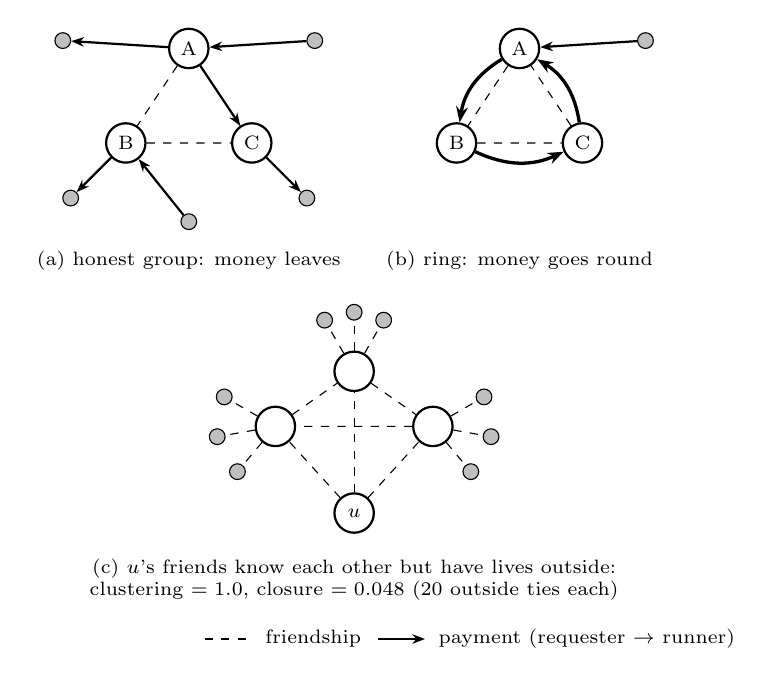
\begin{tikzpicture}[
  font=\scriptsize,
  person/.style={circle, draw, thick, minimum size=5mm, inner sep=0pt},
  other/.style={circle, draw, fill=black!25, minimum size=2mm, inner sep=0pt},
  friend/.style={dashed, thin},
  paid/.style={-{Stealth[length=1.6mm]}, thick},
  ring/.style={-{Stealth[length=2mm]}, very thick}]

  % ---- (a) honest group: money leaves
  \begin{scope}
    \node[person] (a1) at (0,0.9) {A};
    \node[person] (b1) at (-0.8,-0.3) {B};
    \node[person] (c1) at (0.8,-0.3) {C};
    \draw[friend] (a1) -- (b1) -- (c1) -- (a1);
    \node[other] (x1) at (-1.6,1.0) {};  \node[other] (x2) at (1.6,1.0) {};
    \node[other] (x3) at (-1.5,-1.0) {}; \node[other] (x4) at (1.5,-1.0) {};
    \node[other] (x5) at (0,-1.3) {};
    \draw[paid] (a1) -- (x1); \draw[paid] (x2) -- (a1);
    \draw[paid] (b1) -- (x3); \draw[paid] (c1) -- (x4);
    \draw[paid] (x5) -- (b1); \draw[paid] (a1) -- (c1);
    \node at (0,-1.8) {(a) honest group: money leaves};
  \end{scope}

  % ---- (b) ring: money goes round
  \begin{scope}[xshift=4.2cm]
    \node[person] (a2) at (0,0.9) {A};
    \node[person] (b2) at (-0.8,-0.3) {B};
    \node[person] (c2) at (0.8,-0.3) {C};
    \draw[friend] (a2) -- (b2) -- (c2) -- (a2);
    \draw[ring] (a2) to[bend right=25] (b2);
    \draw[ring] (b2) to[bend right=25] (c2);
    \draw[ring] (c2) to[bend right=25] (a2);
    \node[other] (y1) at (1.6,1.0) {};
    \draw[paid] (y1) -- (a2);
    \node at (0,-1.8) {(b) ring: money goes round};
  \end{scope}

  % ---- (c) closure versus clustering
  \begin{scope}[yshift=-4.1cm, xshift=2.1cm]
    \node[person] (u) at (0,-0.9) {$u$};
    \node[person] (p) at (-1.0,0.2) {};
    \node[person] (q) at (0,0.9) {};
    \node[person] (r) at (1.0,0.2) {};
    \draw[friend] (u) -- (p); \draw[friend] (u) -- (q); \draw[friend] (u) -- (r);
    \draw[friend] (p) -- (q) -- (r) -- (p);
    \foreach \n/\ang in {p/150, p/190, p/230, q/60, q/90, q/120, r/-10, r/30, r/-50} {
      \node[other] (o\n\ang) at ($(\n)+(\ang:0.75)$) {};
      \draw[friend] (\n) -- (o\n\ang);
    }
    \node[align=center] at (0,-1.75) {(c) $u$'s friends know each other but have lives outside:\\
      clustering $=1.0$, closure $=0.048$ (20 outside ties each)};
  \end{scope}

  % legend
  \begin{scope}[yshift=-6.6cm, xshift=0.2cm]
    \draw[friend] (0,0) -- (0.6,0); \node[anchor=west] at (0.65,0) {friendship};
    \draw[paid] (2.2,0) -- (2.8,0); \node[anchor=west] at (2.85,0) {payment (requester $\to$ runner)};
  \end{scope}
\end{tikzpicture}

\caption{(a) and (b) are isomorphic friendship triangles; only the payments differ.
(c) A neighbourhood the clustering coefficient scores as fully cohesive but that is
open to the rest of campus.}
\label{fig:shapes}
\end{figure}

\subsection{From Capacity to Evidence: Money Cycles Among Friends}\label{sec:design-rings}
Structure cannot separate three roommates who take turns fetching dinner from three
students farming ratings off each other: the two subgraphs are isomorphic
(Fig.~\ref{fig:shapes}(a), (b)). What differs is whether value circulates.

The \emph{circulation} $\kappa_u$ of a student is the share of the value they moved
on the platform in the last 180 days, in either direction, that moved between them
and their own friends. It is set to 0 below Rs.~300 or four payments, so a newcomer
whose first two errands were for a friend is not read as wholly internal. The
corroboration term in~\eqref{eq:penalty} is $g(\kappa)=\min\bigl(1,(\kappa-0.6)/0.4\bigr)$
for $\kappa>0.6$ and 0 otherwise. Circulation only discounts trust; it accuses nobody.

An accusation needs a closed money cycle. For every ordered pair of mutual friends
$(a,b)$ we total the value $V_{ab}$ and count the distinct errands $n_{ab}$ on edges
$a\to b$ in the window. A leg qualifies if
\begin{equation}
n_{ab}\ge2 \quad\text{and}\quad \bigl(V_{ab}\ge\Rs150 \ \text{or}\ n_{ab}\ge5\bigr).
\end{equation}
The frequency branch closes a loophole: fees may be zero, and a ring that cycles
zero-rupee errands still buys completed errands and ratings. Qualifying legs form a
directed graph, and every strongly connected component with at least three members,
found by an iterative form of Tarjan's algorithm \cite{tarjan1972depth}, is a ring
of any size. Every such component is reported; an earlier version returned only the
50 of highest value, which on a busy campus would have hidden the rest until the
larger ones aged out. Filtering legs before the search matters: if a minimum were
taken over a whole component afterwards, a ring could hide behind one deliberate
Rs.~1 payment.
Every member of a ring is flagged, because a cycle is symmetric and names no
ringleader. No money is withheld, because the cycle identifies a group, not a
dishonest errand.

Why is a cycle suspicious at all, when the platform injects no money and a pure
cycle is zero-sum? Because the motive is cost avoidance. Farming ratings needs
completed errands, each paid for by a confederate. When $A$ pays $B$, $B$ pays $C$
and $C$ pays $A$, each has paid out about what they received, and the group has
produced three completed errands and three ratings at almost no net cost. The money
taken from strangers comes later, through the rank those ratings buy. An honest
friend group's money leaks out to the rest of campus, and for them an internal errand
remains a real expense.

\subsection{Separating the Router's Influence From the Group's Choice}\label{sec:design-policy}
Because dispatch offers errands to friends first, an honest close group produces
money cycles too. Before a ring flag is raised, we ask how much of the group's
in-group activity the routing itself predicts (Fig.~\ref{fig:policy}).

\emph{The acceptance model.} For each logged round $j$ with candidate set $K_j$
($|K_j|\ge2$), the chance that candidate $k$ is the one who accepts is a conditional
logit \cite{mcfadden1974conditional}:
\begin{equation}
p_{jk} = \frac{\exp(\beta^{\top}f_{jk})}{\sum_{l\in K_j}\exp(\beta^{\top}f_{jl})},
\label{eq:logit}
\end{equation}
where $f_{jk}$ holds four logged features: distance in kilometres, whether $k$ is a
direct friend of the requester, whether $k$ is a friend of a friend, and $k$'s
reputation above the neutral 3.5. The weights $\beta$ are fitted by maximum
likelihood (Newton's method with a small ridge term, $10^{-2}$) on every round in
the window whose acceptor was among its candidates, \emph{excluding rounds posted by
a member of any candidate ring}, so a group never helps calibrate the model that
judges it. With fewer than 200 such rounds the model is not trusted, and the test
falls back to the router's own logged scores $e_{jk}$, using
$p_{jk}\propto\exp(-e_{jk}/\theta)$ with $\theta=300$~m. That fallback was the
original design, and Section~\ref{sec:eval-policy} shows why it failed.

\emph{The test.} For the rounds posted by members of the group $S$, let
$\rho_j=\sum_{k\in K_j\cap S}p_{jk}$ be the predicted chance that a member took round
$j$, and let $O$ count the rounds a member actually took. Treating rounds as
independent trials with different probabilities, the count is Poisson-binomial
\cite{wang1993number}, with expectation $E=\sum_j\rho_j$ and variance
$V=\sum_j\rho_j(1-\rho_j)$, and
\begin{equation}
z = \frac{O-E}{\sqrt{V}}. \label{eq:z}
\end{equation}
If $V$ is numerically zero, every round was a foregone conclusion: $z=0$ when $O$
matches $E$, and otherwise $z$ is recorded as $\pm99$, which is never explained. With
at least 25 usable rounds in 180 days and $z<3$, the routing explains the group's
behaviour and the ring flag is suppressed. Otherwise, or with too little history,
the flag stands and goes to a reviewer. The test can only clear; a high $z$ never
raises a severity or creates a flag.

\emph{What the test can and cannot identify.} The model describes how students
\emph{outside} suspected groups respond to being offered an errand by a friend at a
given distance. A ring is separable from honest friends only to the extent that it
takes its own errands more often than such friends do. An honest group that
deliberately routes favours to one another breaks that assumption in exactly the way
a ring does, so no test built on these logs can tell the two apart; only the content
of the errands, or a person, can. We return to this limit in
Section~\ref{sec:discussion}.

A test like this is only informative if some rounds are not shaped by the social
boost. In 5\% of rounds the first offer is \emph{exploratory}: it goes to the five
nearest runners with no trust term and no friendship filter, and its scores are
logged without trust. This costs those requesters a less socially matched runner. It
is paid to keep a control group in the data \cite{li2010contextual,bottou2013counterfactual}.

\begin{figure}[!t]
\centering
% Policy-conditioned evidence, left to right. The acceptance model is fitted on
% rounds posted by people outside every candidate ring, then used to predict how
% often the flagged group S should have taken its own errands.
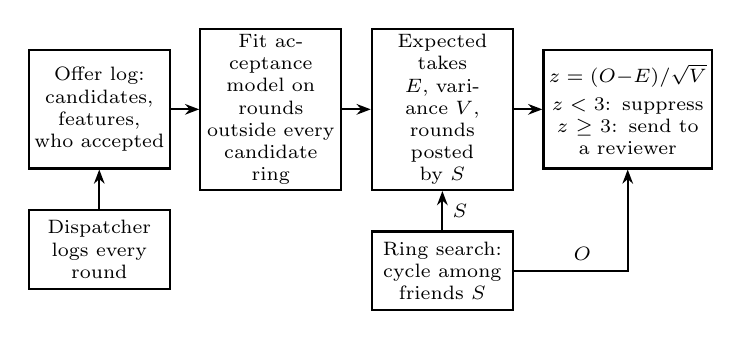
\begin{tikzpicture}[
  font=\scriptsize,
  box/.style={draw, thick, rectangle, align=center, inner sep=2pt, text width=16.5mm,
              minimum height=15mm, fill=white},
  flow/.style={-{Stealth[length=1.8mm]}, thick},
  node distance=3.6mm]
  \node[box] (log) {Offer log:\\candidates, features,\\who accepted};
  \node[box, right=of log] (fit) {Fit acceptance\\model on rounds\\outside every\\candidate ring};
  \node[box, right=of fit] (exp) {Expected takes\\$E$, variance $V$,\\rounds posted\\by $S$};
  \node[box, text width=20mm, right=of exp] (dec)
       {\mbox{$z=(O{-}E)/\sqrt{V}$}\\[2pt]$z<3$: suppress\\$z\ge3$: send to\\a reviewer};
  \node[box, minimum height=10mm, below=5mm of log] (disp) {Dispatcher\\logs every round};
  \node[box, minimum height=10mm, below=5mm of exp] (ring) {Ring search:\\cycle among\\friends $S$};
  \draw[flow] (log) -- (fit);
  \draw[flow] (fit) -- (exp);
  \draw[flow] (exp) -- (dec);
  \draw[flow] (disp) -- (log);
  \draw[flow] (ring) -- node[right] {$S$} (exp);
  \draw[flow] (ring.east) -| node[pos=0.3, above] {$O$} (dec.south);
\end{tikzpicture}

\caption{Policy-conditioned evidence, read left to right. An acceptance model fitted
on rounds posted outside every candidate ring predicts how often the flagged group
$S$ should have taken its own errands; only the unexplained excess is evidence.}
\label{fig:policy}
\end{figure}

\subsection{Reputation That Counts People, Not Ratings}\label{sec:design-reputation}
Errandly keeps two numbers per runner. The plain average is what a student sees on a
profile. Ranking uses a provenance-weighted score. For runner $v$, let the
\emph{concentration} $\phi$ be the share of $v$'s ratings given by $v$'s friends.
Each distinct rater $i$ casts one vote $\bar r_i$, the mean of their ratings, with
weight
\begin{equation}
w_i = \begin{cases}1-\min\bigl(0.75,\ 1.5\,(\phi-0.5)\bigr), & i\in N(v),\ \phi>0.5,\\
1, & \text{otherwise.}\end{cases}
\end{equation}
The score $\bar s=\sum_i w_i\bar r_i/\sum_i w_i$ is shrunk toward a neutral 3.5 by the
effective sample size $W=\sum_i w_i$:
\begin{equation}
m = \frac{W}{W+8}\,\bar s + \frac{8}{W+8}\times3.5 .
\end{equation}
The discount attaches to concentration, never to friendship: twenty strangers and
five friends leave $v$ untouched. A reputation carried by $v$'s own circle becomes
low-confidence rather than low, and climbing back requires strangers. Counting people
instead of ratings removes the patience exploit; under per-rating weights, 100 farmed
ratings from friends outscored 20 honest ones from strangers.

Three detectors raise a \code{RATING\_FARMING} flag for review once a runner has at
least four in-cluster ratings and a concentration of at least 0.70: friends rating
$v$ at least 0.8 stars higher than at least three strangers do; at least two
high in-cluster ratings within 14 days of a penalty; or at least 15 in-cluster
ratings with at most one from outside and at least 2.5 ratings per friend, the
pattern of a runner who builds standing inside a circle before meeting a victim.

\subsection{Dispatch: Staging Offers in Time}\label{sec:design-dispatch}
Candidates come from a Redis geospatial index. Each is scored in metres of
\emph{effective distance}, so the four terms can be compared directly:
\begin{equation}
e = d - 1500\,T - 800\,(m-3.5) + P, \label{eq:effective}
\end{equation}
where $d$ is distance to the drop point, $T$ is trust from~\eqref{eq:trust}, $m$ the
weighted reputation and $P$ an integrity penalty for open, unreviewed flags: 300, 700
or 1200~m by severity, decaying linearly over 30 days and capped at 2000~m. The cap is
deliberate. Without it, open flags would add up until the penalty exceeded any
plausible distance, turning a demotion into a ban that no human decided. An errand is
also never offered to a runner who shares an open ring flag with that requester.

Sorting is not enough. Every candidate in a round is notified within milliseconds,
so ordering a simultaneous broadcast leaves a race that the nearest stranger often
wins. Errandly stages offers in time instead (Fig.~\ref{fig:dispatch}). The first
round goes to the runners among the five nearest within 3~km who are within two
friendship hops. The scheduler, sweeping every 30~s, widens the offer after 45~s to
four hops among the ten nearest and after 90~s to anyone among the ten nearest within
8~km. If nobody within two hops is near when the errand is posted, the first round
goes straight to the five nearest, because an errand nobody sees is worse than one a
stranger takes, and the 90~s widening to 8~km still applies to it. (In the first
version it did not, and such errands expired more often; Section~\ref{sec:eval-dispatch}.) When the graph cannot answer, every function returns \code{None}
rather than an empty set, and \code{None} filters out nobody.

\begin{figure}[!t]
\centering
% Staged dispatch. Offers widen in time rather than being sorted inside one
% simultaneous broadcast. Earlier offers stay open until someone accepts or
% the errand expires.
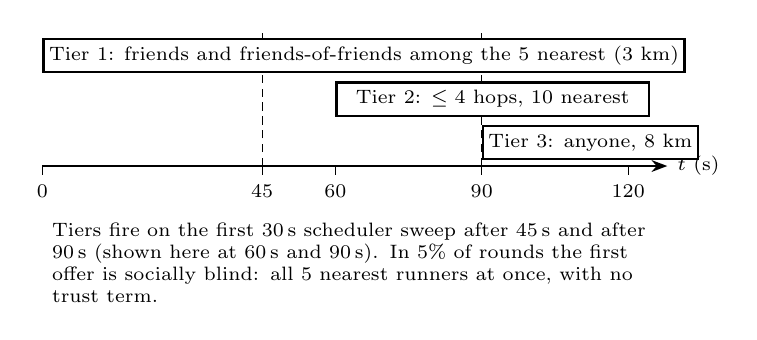
\begin{tikzpicture}[
  font=\scriptsize,
  bar/.style={draw, thick, minimum height=4.2mm, anchor=west, align=left, inner sep=2pt, fill=white},
  x=0.62mm]
  \draw[densely dashed] (45,0) -- (45,17.5mm);
  \draw[densely dashed] (90,0) -- (90,17.5mm);
  \draw[thick, -{Stealth[length=2mm]}] (0,0) -- (128,0) node[right] {$t$ (s)};
  \foreach \t in {0, 45, 60, 90, 120} {
    \draw (\t,0) -- (\t,-1.2mm) node[below] {\t};
  }
  \node[bar, minimum width=124*0.62mm] at (0,14mm)
       {Tier 1: friends and friends-of-friends among the 5 nearest (3 km)};
  \node[bar, minimum width=(124-60)*0.62mm] at (60,8.5mm) {Tier 2: $\le 4$ hops, 10 nearest};
  \node[bar, minimum width=(124-90)*0.62mm] at (90,3mm) {Tier 3: anyone, 8 km};
  \node[align=left, anchor=north west, text width=76mm] at (0,-6mm)
       {Tiers fire on the first 30\,s scheduler sweep after 45\,s and after 90\,s (shown here at
        60\,s and 90\,s). In 5\% of rounds the first offer is socially blind: all 5 nearest
        runners at once, with no trust term.};
\end{tikzpicture}

\caption{Staged dispatch. Social preference comes from when each circle is told,
not from the order of a single broadcast.}
\label{fig:dispatch}
\end{figure}

\subsection{Escrow With Targeted Headroom}\label{sec:design-escrow}
A runner who fronts cash at the counter relies on the hold existing, so it is placed
before any offer:
\begin{equation}
H = X + C + 0.16\,X_{\text{loose}} + F,
\end{equation}
where $X$ is the priced item total, $C$ the cash to collect, $X_{\text{loose}}$ the
subtotal of loose-priced items at their references and $F$ the fee. Only the
loose-priced part gets headroom, because a menu price or a printed MRP is already
known. At settlement the runner is paid the fee and the eligible reimbursement; any
surplus returns to the requester at once. If what the runner is owed exceeds the
remaining hold, the payout is frozen for an administrator, because paying in full
would charge the requester more than they agreed to lock, and paying the capped
amount would make the runner absorb a gap that may be a genuine price rise.
Balances are never stored; a balance is a sum over an append-only ledger, and a
uniqueness constraint on (errand, user, entry type) makes a redelivered settlement
event a no-op.

\subsection{The Language Channel}\label{sec:design-llm}
Structure and money answer \emph{who} and \emph{how much}; neither answers
\emph{what for}. When a ring flag is raised, a locally hosted model reads the errand
texts of the group and returns a schema-constrained assessment for the reviewer. The
channel is advisory: it never raises a severity, never withholds money and never
creates a flag. Its useful direction is exculpatory, where being wrong costs least.
All text is fenced and labelled as untrusted, and the output schema leaves a crafted
note nothing to do but move a number a human can see \cite{greshake2023not}. A second
channel that reads rating comments is switched off, for the reason given in
Section~\ref{sec:eval-system}.

\begin{table}[!t]
\caption{Main Parameters of the Deployed System}
\label{tab:params}
\centering
\footnotesize
\begin{tabular}{@{}>{\raggedright}p{0.52\columnwidth}>{\raggedright\arraybackslash}p{0.38\columnwidth}@{}}
\toprule
Parameter & Value \\
\midrule
Allowance on a loose item & 40\% of reference, Rs.~5 to Rs.~20 \\
Near-line rule & $\ge0.6\,\tau$; $\ge4$ claims and $\ge60\%$ \\
Strike ladder (flagged errands, 30 days) & 3 / 5 / 8 open; 12 upheld \\
Reference estimate & $\ge3$ runners, $\ge5$ claims; cut at $3\times1.4826$ MAD \\
Shop pooling & prior 6; $\ge3$ runners \\
Trust hop decay $\delta$; maximum hops & 0.45; 4 \\
Friendship maturity & 30 days; floor 0.40 \\
Closure knee; structural / corroborated cap & 0.55; 0.70 / 0.95 \\
Circulation knee; evidence floor & 0.60; Rs.~300 and 4 payments \\
Money window & 180 days \\
Ring leg & $\ge2$ errands and ($\ge$Rs.~150 or $\ge5$ errands) \\
Policy test & $\ge25$ rounds; $z<3$ clears \\
Acceptance model & $\ge200$ rounds; ridge $10^{-2}$; else $\theta=300$~m \\
Exploration rate & 5\% of first offers \\
Trust / reputation weight in~\eqref{eq:effective} & 1500~m / 800~m per star \\
Open-flag penalty & 300 / 700 / 1200~m; cap 2000~m \\
Rating concentration knee; maximum discount & 0.50; 0.75 \\
Rating confidence prior & 8 ratings at 3.5 \\
Escrow headroom & 16\% of loose-priced subtotal \\
\bottomrule
\end{tabular}
\end{table}


%======================================================================
\section{Implementation}\label{sec:impl}
%======================================================================

The backend is about 12,900 lines of Python 3.12 using FastAPI and SQLAlchemy 2.0
(asynchronous), with PostgreSQL 16 and PostGIS for errands, ledger and fraud data,
Redis 7 for the runner geospatial index, accept locks and publish--subscribe, Kafka
3.8 in KRaft mode as the event backbone, Neo4j 5.26 Community Edition for the
friendship and payment graph, and MongoDB 7 for chat. Twenty-four migrations define
the schema and the API exposes 70 HTTP routes plus WebSocket channels for live
tracking and offers. The student client is built with React Native 0.86 and Expo 57,
and the web client with React 18, TypeScript and Leaflet. The language channel runs
Qwen2.5~7B through Ollama on campus hardware, so no student text leaves the
institution.

Money moves in exactly one place: the settlement consumer, on the completion event.
Two independent gates make Kafka's at-least-once delivery harmless: a
processed-events table at the consumer and the ledger's uniqueness constraint. This
follows the transactional outbox pattern
\cite{richardson2018microservices,kleppmann2017designing}. Graph reads use circuit
breakers \cite{nygard2018release}; a graph outage degrades matching to distance order.
Graph metrics are computed in plain Cypher; we avoided the Graph Data Science plugin,
whose download at container start would make an offline start fail.

We treat explainability as a design rule. Every flag stores the evidence
that raised it: the reference and allowance a claim was held to, the shop and how
many runners have priced it, a ring's members, laps, value and policy statistic.
Every offer round stores the four terms of~\eqref{eq:effective} for every candidate.
These decisions withhold money and suspend students, and an accusation that cannot be
explained cannot be contested \cite{goodman2017european}. This is also why learned
models are confined to the advisory channel.

\emph{Changes made after the first evaluation.} The first round of experiments
exposed six faults, and each was fixed in the production code, with a regression
test, before the results reported here were produced. (i) A claim could be renamed
until it matched no reference and was then paid unchecked; claims are now bound to
the order's own lines, and quantities are capped at the quantity ordered. (ii) The
policy test reused the router's scores as its model of acceptance and cleared
coordinated rings; it now fits an acceptance model to logged acceptances. (iii) When
the predicted probabilities left no variance, the test reported $z=0$ and cleared the
group even when the group had taken rounds it had no predicted chance of taking.
(iv) Errands whose first offer went out unrestricted were never widened. (v) The ring
search returned at most 50 rings. (vi) Unreviewed ring flags counted toward the
automatic strike ladder, and its last step, account suspension, needed no human.
Section~\ref{sec:eval} reports the original behaviour beside the fixed one where the
difference is measurable.

The backend has 273 automated tests (6,014 lines). In an isolated container against
its own database, a separate Redis database and a separate Neo4j instance, all 273
passed in 111~s.

%======================================================================
\section{Evaluation}\label{sec:eval}
%======================================================================

\subsection{Method}\label{sec:eval-method}
There is no pilot data yet, so we evaluate in simulation, and we take care over what
is simulated. The experiment scripts import the production modules unchanged. Only
storage is replaced: database sessions are swapped for small fakes that return
prepared rows, and graph queries run against a separate, disposable Neo4j instance
loaded with the simulated campus. The decision logic, constants and Cypher queries are
the deployed ones. Every number below is regenerated by one script per experiment in
the repository, and every result file records the commit it was produced from, the
seeds and the machine.

\emph{Seeds and intervals.} The collusion, price-claim, dispatch and escrow
experiments use 30 seeds for their main results and 10 seeds per point for parameter
sweeps. We report means with the half-width of a two-sided 95\% confidence interval
of the mean, from the Student $t$ distribution across seeds. A seed fixes the
friendship graph, the planted groups, the homes, who is online, every runner's
willingness and delay, and the exploration coin, so two policies run on the same
seed see the same semester.

\emph{Hardware.} All experiments ran in Docker containers on one laptop with an
Intel Core i7-12650H (10 cores, 16 threads) and 7.6~GiB of memory available to
Docker, with Python 3.12 and Neo4j 5.26 Community Edition. The timing experiment
(Section~\ref{sec:eval-system}) ran alone on the machine; the others ran in
parallel, each against its own Neo4j instance.

The campus has 1,200 students in 24 hostel blocks of 50. Friendships follow a
stochastic block model \cite{holland1983stochastic}, with probability 0.10 within a
block and 0.0015 across blocks, giving a mean degree of 7.2; residence-dominated
community structure of this kind has been observed in real campus networks
\cite{traud2012social}. We plant 28 honest close-knit groups (sizes 3 to 8, 120
students) and five collusion rings (sizes 3, 4, 5, 6 and 8, 26 students), each as a
clique inside one block, so honest groups and rings are structurally identical by
construction. Over a 180-day semester each student posts errands at 0.12 per day;
fees are drawn from Rs.~20--50, and 30\% of errands carry Rs.~50--400 of cash to
collect. Each errand sees a random 12\% of students online. Dispatch uses the
production ranking, tiers, scheduler cadence and exploration coin. An offered runner
accepts with probability $0.5\,e^{-d/2000\,\mathrm{m}}$, multiplied by a friend
affinity of 1.5 for direct friends, after a log-normal delay with median 20~s. These
behavioural parameters are assumptions, which is why we vary them. Ring members each
post 12 extra low-fee errands that a ring partner takes from the feed within
3--15~s.

To check that the simulator dispatched as production would, closure and circulation
computed inside the simulator were compared with the production Cypher on the final
graph of every trial; the largest difference in any trial was 0.

Table~\ref{tab:summary} collects the main results; the subsections that follow give
the detail behind each row.

% Consolidated results. Every entry is regenerated by the script named in the
% last column; see backend/evals/paper/README.md.
\begin{table*}[!t]
\caption{Summary of Results. Mean (95\% CI Half-Width) Unless Stated}
\label{tab:summary}
\centering
\scriptsize
\setlength{\tabcolsep}{3pt}
\begin{tabular}{@{}>{\raggedright}p{0.11\textwidth}>{\raggedright}p{0.31\textwidth}>{\raggedright}p{0.36\textwidth}l@{}}
\toprule
Area & Measure & Result & Runs (script) \\
\midrule
Ring detection, deployed pipeline & F1, routine / busy / favours / coordinated / hard &
0.97 (0.02) / 0.96 (0.02) / 0.93 (0.03) / 0.88 (0.04) / 0.87 (0.04) & 30 seeds (exp2) \\
& Ring members found (TP / FN of 26), same order & 24.7/1.3, 24.9/1.1, 24.4/1.6, 20.7/5.3,
22.1/3.9 & \\
& Cycle search alone (base), F1 routine / coordinated & 0.96 (0.02) / 0.99 (0.01) & \\
& Best graph-mining baseline, F1 & 0.28 to 0.48 (FRAUDAR-style, given the true count) & \\
\midrule
Honest impact & Honest students flagged per trial (of 1,174), same order &
0.2 (0.2), 0.6 (0.4), 1.9 (1.0), 0.0 (0.1), 2.3 (1.0); FPR at most 0.20\% & 30 seeds (exp2) \\
& With 24 honest favours per member & 110 per trial: the identifiability limit & 10 seeds (exp2) \\
\midrule
Policy test & Coordinated-ring recall, router scores vs fitted model & 0.02 (0.02) vs 0.79
(0.06) & 30 seeds (exp2) \\
& Honest-only cycles cleared, busy / favours / hard & 25 of 26, 35 of 50, 28 of 48 & \\
& Adaptive ring, members caught at 4 / 8 / 12 farmed errands & 0\% / 42\% / 86\% & 10 seeds (exp2) \\
\midrule
Price claims & Reference after 16 weeks, any strategy, up to 60\% dishonest & Rs.~20.00 in
every seed (true price Rs.~20) & 30 seeds (exp3) \\
& Honest claims flagged; honest near-line flags & 0 of all honest claims; 0 runners &
4,620 runs (exp3) \\
& Line-walkers at 30\%: days to flag; excess before flag; 16 weeks unreviewed & 19.3
(1.2) days; Rs.~331 (4); Rs.~1,958 (46) & 30 seeds (exp3) \\
& Evasive at 30\%: share flagged; days to flag & 79\%; 46.4 (3.2) days & \\
& Adversarial names paid unchecked, old rule vs deployed & 41 of 61 vs 6 of 61 (all
swaps to an unpriced line) & deterministic (exp9) \\
& Colluders needed to move a shop with 0 / 10 honest reporters & 3 / 10 & deterministic (exp4) \\
\midrule
Dispatch & Errands taken within 2 hops: broadcast / staged / one at a time & 17.8\% / 35.8\% /
50.4\% (all $\pm0.3$) & 30 seeds (exp6) \\
& Median wait to accept, same order & 12.3 / 19.0 / 41.9 s & \\
& Unaccepted after 30 min, staged, original vs fixed scheduler & 1.88\% (0.03) vs 0.22\% (0.01) & \\
\midrule
Escrow & Payouts frozen at 16\% headroom; money locked without need & 9.0\% (0.2);
Rs.~12.7 (0.1) per order & 30 seeds (exp7) \\
\midrule
Runtime & Three graph jobs at 10,000 students; trust lookup p50 / p95 & 11.9 s per sweep;
3.0 / 4.2 ms & 5 repetitions, run alone (exp8) \\
\bottomrule
\multicolumn{4}{@{}p{0.97\textwidth}@{}}{Regimes and attacks are defined in
Sections~\ref{sec:eval-rings} and~\ref{sec:eval-price}. ``Base'' is the cycle search
without the policy test; the deployed pipeline adds the fitted policy test. Hardware:
Intel Core i7-12650H, 16 threads, 7.6~GiB for Docker.}
\end{tabular}
\end{table*}


\subsection{Closure Versus Clustering}\label{sec:eval-closure}
% Experiment 1: backend/evals/paper/exp1_closure.py
Table~\ref{tab:closure} scores canonical neighbourhoods with the production
\code{REFRESH\_METRICS} query on Neo4j and, as a cross-check, with an exact Python
transcription of it; the two agreed on all 425 nodes.

The two measures agree more often than one might expect. On a sealed clique both are
1.0 at every size, and when each clique member has one private friend they give
identical values: 0.50 for four members and 0.80 for ten. Closure is therefore not
size-invariant in general, and we do not claim that it is. Where the measures part
ways is a neighbourhood whose members have lives outside it. When ego's three friends
all know each other but each has twenty friendships elsewhere, the clustering
coefficient is 1.0 and, used in place of closure, would apply the full 0.70 structural
discount. Closure is 0.048 and applies none. In the second-to-last row, counting
ego's own spokes as internal edges would lift the closure of an open hub from 0 to
0.50, which is why the query excludes ego.

\begin{table}[!t]
\caption{Closure Versus the Clustering Coefficient on Canonical Neighbourhoods}
\label{tab:closure}
\centering
\footnotesize
\begin{tabular}{@{}>{\raggedright}p{0.40\columnwidth}cccc@{}}
\toprule
Ego's neighbourhood & $C$ & $c$ & $\pi(C)$ & $\pi(c)$ \\
\midrule
Sealed clique, 3 or 10 members & 1.00 & 1.00 & 0.70 & 0.70 \\
Clique of 4, one private friend each & 0.50 & 0.50 & 0 & 0 \\
Clique of 10, one private friend each & 0.80 & 0.80 & 0.39 & 0.39 \\
Clique of 10, two sociable friends each & 0.66 & 0.56 & 0.16 & 0.02 \\
Friends form a triangle, each with 20 outside ties & 1.00 & 0.05 & 0.70 & 0 \\
Hub, 8 unacquainted friends with one other tie each$^\dagger$ & 0 & 0 & 0 & 0 \\
Sealed sparse group, 10 people with 4 ties each & 0.50 & 0.33 & 0 & 0 \\
\bottomrule
\multicolumn{5}{@{}p{0.95\columnwidth}@{}}{\scriptsize $C$: clustering coefficient;
$c$: closure~\eqref{eq:closure}; $\pi(\cdot)$: structural penalty when that measure is
used. $^\dagger$Counting ego inside its own neighbourhood gives $c=0.50$.}
\end{tabular}
\end{table}


\subsection{Detecting Rings Among Honest Friend Groups}\label{sec:eval-rings}
% Experiment 2 (main table): backend/evals/paper/exp2_collusion.py main <regimes>  (30 seeds)
\emph{Regimes.} We compare ten detectors in five behavioural regimes, 30 seeds each.
In the \emph{routine} regime friends meet only through the router. The \emph{busy}
regime has twice as many runners online and friends four times likelier to accept
each other's offers, so the router itself puts honest friends together. In the
\emph{favours} regime every honest group member also posts six errands per semester
meant for a particular friend, who takes them from the feed; this is deliberate
in-group routing with nothing dishonest about it. In the \emph{coordinated} regime the
rings are careful: before each farming errand the partner comes online and walks
over, so the router offers the errand to the partner first. The \emph{hard} regime
combines honest favours with coordinated rings.

\emph{Detectors.} Four single-signal baselines use structure or money at the
production knees. A cycle baseline applies the ring search's leg rule and
strongly-connected-component search to any pair of students, without the friendship
test. Two graph-mining baselines come from the fraud literature. The first is
FRAUDAR-style greedy peeling \cite{hooi2016fraudar,charikar2000dense} on the
bipartite payer--payee graph, with edges weighted by the number of errands and the
logarithmic column weighting FRAUDAR uses against camouflage. The second is
label-propagation communities \cite{raghavan2007lpa} on the friendship graph, ranked
by the share of their members' value that stays inside. The last three rows are the
ring search and the ring search followed by each version of the policy test.

\begin{table*}[!t]
\caption{Ring Detection on a Simulated 1,200-Student Campus. Precision (P), Recall
(R) and False-Positive Rate (FPR, \%), Mean of 30 Seeds}
\label{tab:rings}
\centering
\scriptsize
\setlength{\tabcolsep}{2.4pt}
\begin{tabular}{@{}lccccccccccccccc@{}}
\toprule
& \multicolumn{3}{c}{Routine} & \multicolumn{3}{c}{Busy} & \multicolumn{3}{c}{Favours}
& \multicolumn{3}{c}{Coordinated} & \multicolumn{3}{c}{Hard} \\
\cmidrule(lr){2-4}\cmidrule(lr){5-7}\cmidrule(lr){8-10}\cmidrule(lr){11-13}\cmidrule(l){14-16}
Detector & P & R & FPR & P & R & FPR & P & R & FPR & P & R & FPR & P & R & FPR \\
\midrule
Closure, circulation, or both & n/a & 0.00 & 0.00 & n/a & 0.00 & 0.03 & n/a & 0.00 & 0.00 & n/a & 0.00 & 0.00 & n/a & 0.00 & 0.00 \\
Clustering coefficient $>0.55$ & 0.11 & 0.03 & 0.44 & 0.11 & 0.03 & 0.44 & 0.11 & 0.03 & 0.44 & 0.11 & 0.03 & 0.44 & 0.11 & 0.03 & 0.44 \\
Payment cycles, any pair & 0.63 & 0.95 & 1.34 & 0.38 & 0.96 & 3.73 & 0.50 & 0.94 & 2.23 & 0.69 & 0.99 & 1.12 & 0.48 & 0.99 & 2.48 \\
FRAUDAR-style peeling$^{\dagger}$ & 0.36 & 0.36 & 1.41 & 0.28 & 0.28 & 1.59 & 0.30 & 0.30 & 1.55 & 0.48 & 0.48 & 1.16 & 0.43 & 0.43 & 1.27 \\
Label propagation + money$^{\dagger}$ & 0.03 & 0.06 & 4.18 & 0.02 & 0.03 & 4.17 & 0.02 & 0.04 & 4.30 & 0.01 & 0.02 & 4.21 & 0.03 & 0.05 & 4.15 \\
Cycles among mutual friends (\code{find\_rings}) & 0.98 & 0.95 & 0.05 & 0.89 & 0.96 & 0.29 & 0.82 & 0.94 & 0.50 & 0.99 & 0.99 & 0.03 & 0.83 & 0.99 & 0.47 \\
\quad + policy test, router scores (original) & 0.99 & 0.95 & 0.02 & 0.98 & 0.96 & 0.05 & 0.94 & 0.94 & 0.13 & 0.10 & 0.02 & 0.00 & 0.15 & 0.04 & 0.17 \\
\quad + policy test, fitted model (deployed) & 0.99 & 0.95 & 0.02 & 0.98 & 0.96 & 0.05 & 0.93 & 0.94 & 0.16 & 1.00 & 0.79 & 0.00 & 0.91 & 0.85 & 0.20 \\
\bottomrule
\end{tabular}

\vspace{2pt}
\parbox{0.96\textwidth}{\scriptsize Recall is over the 26 planted ring members; FPR is
over the 1,174 other students. Precision is counted as 0 in a trial that flags nobody;
``n/a'' marks detectors that flagged nobody in almost every trial. Structure is the same
in every regime, so the clustering row repeats. $^{\dagger}$Scored as a ranking cut at
the true number of ring members, which no deployment would know. Half-widths of 95\%
confidence intervals are at most 0.06 for precision or recall in the last three rows
and at most 0.12 elsewhere; Table~\ref{tab:summary} gives them for the deployed
detector.}
\end{table*}

\emph{Single signals see nothing.} Ring members, like everyone, have friends outside
their ring, so their closure stays under the 0.55 knee; and because farming errands
are cheap and members keep running ordinary errands, circulation stays under 0.6. The
clustering coefficient flags about five students per trial, mostly honest group
members, and almost never a ring member.

\emph{Graph-mining baselines find the marketplace, not the ring.} FRAUDAR's own
output, its densest block, was the whole campus (1,199 or 1,200 accounts) in every
trial. A ring of three to eight students who each run a dozen cheap errands for one
another is not dense compared with the core of an active marketplace, where everyone
pays everyone a little. Cut at the true number of ring members, the peeling order
still reached an F1 score of only 0.28--0.48. Label-propagation communities were about
the size of a hostel block, so no community crossed the circulation knee in any trial,
and the ranked version mostly flagged a whole block of honest students. Both methods
look for large dense or tightly-knit groups. The groups we are after are small, and
dense only in money that flows around a cycle.

\emph{Cycles need the friendship test.} Payment cycles without the friendship test
found almost every ring member but flagged 13 to 44 honest students per trial,
because repeated errands between nearby strangers also close cycles. Requiring every
leg to join mutual friends is what makes cycle evidence usable: \code{find\_rings}
reached an F1 score of $0.96\pm0.02$ in the routine regime and $0.99\pm0.01$ against
coordinated rings, which do not change the money pattern.

\emph{The router's false positives.} The ring search's false positives come from the
two cases it cannot see through: router-induced cycles (3.4 honest students per trial
in the busy regime) and honest favours (5.9 in the favours regime, 5.5 in the hard
one). Both versions of the policy test removed most of them. The fitted test removed
82\% in the busy regime and 68\% with honest favours, lifting F1 from 0.92 to 0.96 and
from 0.87 to 0.93, and lost no ring member in either.

\emph{Where the original test failed.} Against coordinated rings the router-score
test cleared 146 of the 149 cycles that contained ring members, and recall fell from
0.99 to 0.02. The fitted test cleared 37 of them, for a recall of $0.79\pm0.06$ at a
precision of 1.00. With honest favours added (the hard regime) the original test kept
a recall of 0.04 and the fitted test 0.85, at a precision of 0.91.
Section~\ref{sec:eval-policy} examines why.

\emph{Variability.} Recall below 1 in the routine, busy and favours regimes came from
seeds in which honest runners won enough of a ring's cheap errands to push one leg
under the qualification floor (on average 1.3 of 26 members missed in the routine
regime). Fig.~\ref{fig:sweeps}(b) shows how that floor depends on farming intensity.
The number of cycles raised per trial varied from four to nine, because some seeds
plant honest groups where the router closes a cycle.


\subsection{Separating Routing From Choice}\label{sec:eval-policy}
% Experiment 2 (statistics and sweeps): backend/evals/paper/exp2_collusion.py
%   main: 30 seeds per regime; sweeps explore / weight_favours / intensity_adaptive: 10 seeds
Fig.~\ref{fig:z} plots the policy statistic~\eqref{eq:z} for every planted group in the
main runs, under both acceptance models.

\emph{Reading Fig.~\ref{fig:z}.} Each marker is one planted group in one trial. An
open circle is an honest close-knit group and a filled square is a collusion ring.
Each regime has one column: up to 840 honest groups (28 per seed over 30 seeds) and
150 rings (5 per seed). Markers are spread sideways only so that they do not hide one
another; the horizontal position inside a column carries no meaning. The vertical
axis is $z$, how many standard deviations a group's in-group takes lie above what the
acceptance model predicted. At $z=0$ the group did exactly what the model expected;
a positive $z$ means its members took one another's errands more often than
predicted. The horizontal line at $z=3$ is the decision threshold. If the ring search
flags a group below the line, the test clears it; a group above the line goes to a
reviewer. The two numbers above each column count the honest groups (top) and rings
(bottom) on or above the line. A good test puts the circles below the line and the
squares above it. Panel (a) does this in the routine and busy regimes but not with
coordinated rings, whose squares sit among the circles. In panel (b) those squares
rise above the line while the circles stay near zero. In the favours and hard
columns, many circles cross the line in both panels: honest groups that deliberately
route favours look like rings to any test built on these logs.

\emph{Calibration.} With the router's scores (Fig.~\ref{fig:z}(a)), honest groups in
the routine regime had a median $z$ of $-2.1$: the router's scores predict more
in-group takes than honest groups make, because every candidate in a tier is told at
once and the order of the list matters little. The fitted model
(Fig.~\ref{fig:z}(b)) centres honest groups near zero (median $-0.2$), which is what
a calibrated test should do. Its weights describe the simulated behaviour as one would
hope: averaged over seeds, a kilometre of distance cost 0.65 in log-odds and being a
direct friend added 0.51, rising to 0.97 in the busy regime, where friends were
simulated as four times likelier to accept. Friend-of-friend status added almost
nothing ($-0.03$), and reputation is constant in the simulation, so its weight is
zero.

\emph{Separation.} In the routine and busy regimes both versions separated cleanly:
every ring and at most 1\% of honest groups reached $z=3$. Against coordinated rings
they part ways. With the router's scores only 3 of 150 rings reached the line (median
$z=0.4$), because a partner who is always the router's first pick looks, to a test
that trusts the router, like the router's own doing. With the fitted model 112 of 150
did (median 3.7). A friend who takes a group's errands every time is unusual compared
with how friends elsewhere on campus behave, and that comparison is what the fitted
model makes.

\emph{Honest favours.} When honest groups deliberately route favours to each other,
34\% of them exceeded $z=3$ under the router's scores and 42\% under the fitted model,
because the fitted model no longer starts from a conservative margin. The test only
acts on groups the ring search raised, though, and of the 50 honest-only cycles
raised in the favours regime it cleared 35 (the router-score version cleared 37).

\begin{figure}[!t]
\centering
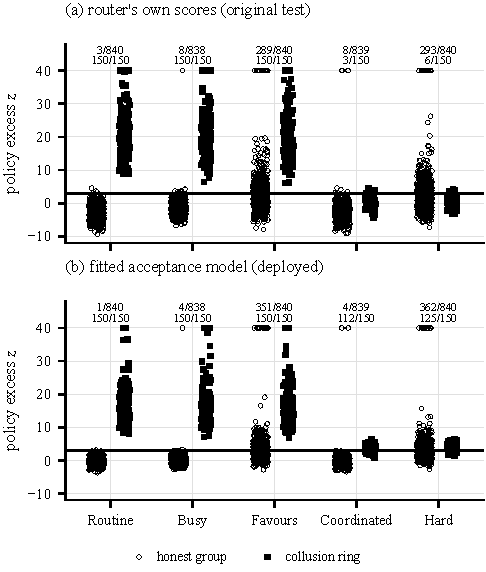
\includegraphics[width=\columnwidth]{figures/fig_z.pdf}
\caption{Policy statistic $z$ for every planted group in the main runs (30 seeds per
regime; 28 honest groups and 5 rings per seed) under (a) the router's own logged scores
and (b) the fitted acceptance model. Numbers above each column count honest groups
(top) and rings (bottom) with $z\ge3$, which the test does not clear. Values above 40,
including the $\pm99$ of the degenerate case, are drawn at 40.}
\label{fig:z}
\end{figure}

\emph{Exploration.} Fig.~\ref{fig:explore} varies the exploration rate, ten seeds per
point. The router-score test needed exploration to see coordinated rings at all: its
recall was 0.03 at the deployed 5\%, 0.38 at 20\% and 0.88 at 40\%. The fitted test did
not. Its recall was 0.84 with no exploration, 0.86 at 5\% and 0.98 at 40\%, because it
learns from variation across the whole campus, not from the exploratory rounds of the
group under test. In the busy regime both versions held false positives under one
honest student per trial at every rate, against 1.1 to 3.8 for the ring search alone.
Since exploration costs service (Section~\ref{sec:eval-dispatch}), the fitted model
removes the main reason to raise it.

\emph{Reading Fig.~\ref{fig:explore}.} The horizontal axis of both panels is the
exploration rate, the share of first offers sent without the social boost; the dotted
vertical line marks the deployed 5\%. Panel (a) measures recall against coordinated
rings: the share of the 26 ring members still flagged after the policy test. The
dashed line with open circles is the ring search alone, an upper bound, because the
test can only remove flags, never add them. The dotted line with triangles is the
original test, using the router's scores, and the solid line with filled squares is
the deployed test, using the fitted model. The vertical gap between the dashed line
and a test's line is the share of ring members that test wrongly cleared. The
original test closes that gap only at 40\% exploration; the fitted test stays close
to it at every rate. Panel (b) counts honest students falsely flagged per trial in
the busy regime, where the router itself puts honest friends together, so lower is
better. Here the dashed line shows how many flags the router causes, and the two test
lines show how many remain. Each point is the mean over ten seeds, and its error bar
is the 95\% confidence interval of that mean. The bars in panel (b) are wide because
false positives are few and vary from seed to seed between zero and a handful.

\begin{figure}[!t]
\centering
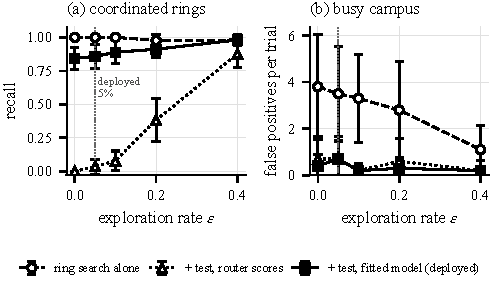
\includegraphics[width=\columnwidth]{figures/fig_explore.pdf}
\caption{Effect of the exploration rate. (a) Recall against coordinated rings. (b)
Honest students falsely flagged per trial in the busy regime. Mean and 95\% confidence
interval over ten seeds; the dotted line marks the deployed rate.}
\label{fig:explore}
\end{figure}

\emph{Trust weight.} The trust weight in~\eqref{eq:effective} changed nothing about
who accepted in our simulation: in-group shares and ring-search results were identical
at 0, 1500 and 3000~m, because every runner in a tier is told at the same moment. It
did change what the router-score test expected. With the weight at zero that test kept
97\% of coordinated ring members flagged, and at 1500 or 3000~m it kept 3\%. The fitted
test kept 86\% at all three weights, because it never reads the router's weights.

\emph{The two limits.} Fig.~\ref{fig:sweeps} shows where relational evidence stops.
As honest groups trade more favours (panel a), the ring search flags more of them:
0.1, 1.9, 7.8, 37.6 and 112.6 honest students per trial at 0, 3, 6, 12 and 24 favours
per member. The fitted test cleared 63\% of these at three favours per member and 76\%
at six, but only 27\% at twelve and 2\% at twenty-four. That much deliberate in-group
routing is beyond what ordinary friends do, and the test is right to say so; what it
cannot say is that the routing was innocent. Panel (b) shows the other end. Because a
leg must carry at least five errands or Rs.~150, and honest runners sometimes take a
ring's errand first, the ring search found almost no ring member when rings farmed
four or fewer errands per member in a semester, 47\% at eight and 97\% at twelve. The
\emph{adaptive} attacker, a coordinated ring that chooses how much to farm, adds the
policy test's own floor: against it the deployed pipeline caught 42\% of members at
eight errands, 86\% at twelve and all of them at twenty-four. Below that floor the
pipeline is blind, but the farming is also small: at four errands per member the five
rings together moved about Rs.~1,600 in a semester, and under one vote per rater a
member farming from three partners gets three votes however many errands they run
(Section~\ref{sec:eval-farming}).

\emph{Reading Fig.~\ref{fig:sweeps}.} In panel (a) the horizontal axis is the number
of favours each honest group member deliberately routes to a friend in a semester,
and the vertical axis is the number of honest students flagged per trial. The three
lines use the same markers as Fig.~\ref{fig:explore}. The gap between the dashed line
(ring search alone) and the solid line (deployed test) is the honest flags that the
test clears. That gap is wide at three and six favours, narrows at twelve and all but
closes at twenty-four, where the lines meet: there the test, correctly by its own
definition, finds the routing unexplained. In panel (b) the horizontal axis is the
number of farmed errands per ring member in a semester, and the vertical axis is
recall. The dashed line is careless (routine) rings against the ring search alone;
where it rises shows the qualification floor of a payment leg. The solid line is
coordinated rings, which choose their own volume, against the deployed pipeline;
where it rises shows how much an adaptive ring can farm before it is caught. The
point where a curve leaves zero is the volume a ring can stay under. Error bars are
95\% confidence intervals over ten seeds; they are widest at eight errands, where
whether a ring is caught depends on chance in individual seeds.

\begin{figure}[!t]
\centering
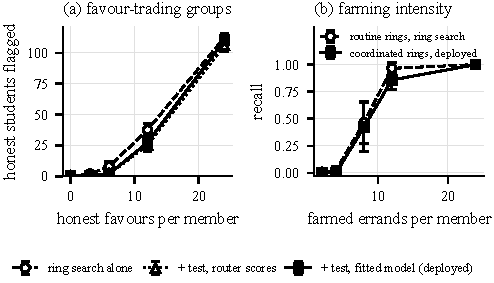
\includegraphics[width=\columnwidth]{figures/fig_sweeps.pdf}
\caption{(a) Honest students flagged as honest favour-trading grows (legend below).
(b) Recall as rings farm fewer errands: careless rings against the ring search, and
coordinated rings, which choose their volume, against the deployed pipeline. Mean and
95\% confidence interval over ten seeds.}
\label{fig:sweeps}
\end{figure}


\subsection{Reference Prices Under Attack}\label{sec:eval-price}
% Experiment 3: backend/evals/paper/exp3_reference.py   (30 seeds)
% Experiment 4: backend/evals/paper/exp4_store.py       (deterministic)
% Experiment 9: backend/evals/paper/exp9_normalize.py   (adversarial names)
\emph{Setup.} We simulated 16 weeks of claims for one item, a chicken puff with an
administrator reference of Rs.~20 and band Rs.~15--30, from 40 runners filing about
1.5 claims a week. Honest runners report Rs.~20, or Rs.~22 on the 15\% of days the
canteen charges more. Dishonest runners follow one of four strategies: \emph{line},
claiming 95\% of the allowance above the reference every time; \emph{evasive}, doing
so on a random half of their claims, intending to stay under the 60\% share the
near-line rule requires; \emph{overt}, claiming Rs.~30; and \emph{volume}, one runner
claiming at the line ten times as often as anyone else. The reference is
re-estimated weekly, and every claim is judged by the production code against the
reference in force when it was made. Each configuration was run with 30 seeds, and
we report the mean with the half-width of a 95\% confidence interval.

\begin{table*}[!t]
\caption{Reference Price (Rs.) After 16 Weeks, by Estimator and Attack.
Mean (95\% CI Half-Width) Over 30 Seeds}
\label{tab:reference}
\centering
\footnotesize
\setlength{\tabcolsep}{5pt}
\begin{tabular}{@{}lcccccc@{}}
\toprule
& \multicolumn{3}{c}{Line-walking} & Evasive & Overt & Volume \\
\cmidrule(lr){2-4}\cmidrule(lr){5-5}\cmidrule(lr){6-6}\cmidrule(l){7-7}
Dishonest runners & 30\% & 50\% & 60\% & 60\% & 60\% & 1 of 40 \\
\midrule
Mean, all claims & 24.14 (0.19) & 30.97 (0.40) & 37.80 (0.61) & 24.06 (0.18) & 26.06 (0.10) & 22.35 (0.12) \\
Mean, unflagged & 24.14 (0.19) & 30.97 (0.40) & 37.80 (0.61) & 24.06 (0.18) & 20.33 (0.02) & 22.35 (0.12) \\
Median, unflagged & 20.00 (0) & 31.27 (4.50) & 70.00 (0) & 20.00 (0) & 20.00 (0) & 20.00 (0) \\
One vote per runner & 20.00 (0) & 28.82 (0.97) & 96.96 (3.05) & 20.26 (0.26) & 20.00 (0) & 20.00 (0) \\
\quad + line-walkers excluded & 20.00 (0) & 20.00 (0) & 20.00 (0) & 20.00 (0) & 20.00 (0) & 20.00 (0) \\
\quad + band only & 20.00 (0) & 28.54 (0.91) & 27.50 (0.38) & 20.26 (0.26) & 20.00 (0) & 20.00 (0) \\
Deployed (both) & 20.00 (0) & 20.00 (0) & 20.00 (0) & 20.00 (0) & 20.00 (0) & 20.00 (0) \\
\bottomrule
\multicolumn{7}{@{}l@{}}{\scriptsize True price: Rs.~20, or Rs.~22 on dear days.
``(0)'' means every seed gave the same value.}
\end{tabular}
\end{table*}

\emph{The reference.} Table~\ref{tab:reference} shows three defences doing three
different jobs. Excluding flagged claims stops overt inflation: the mean of all claims
rose to Rs.~26.06 because flagged claims kept voting, while the mean of unflagged
claims stayed near the true price. One vote per runner stops volume: a single runner
filing ten times as often moved either mean by 12\% and no median at all. Against
line-walking, whose claims are never flagged, the vote limit is not enough on its
own. The median-based estimators held with 30\% dishonest runners and broke at 50\%,
and the one-vote estimator, whose allowance grows with the reference, ran away to
Rs.~96.96 at 60\% (Fig.~\ref{fig:reference}). The band bounded that drift. What held
the reference at Rs.~20 in every one of the 30 seeds was the exclusion of runners
under a near-line flag. Across all 4,620 runs no honest runner received a near-line
flag and no honest claim was judged FLAGGED.

\begin{figure}[!t]
\centering
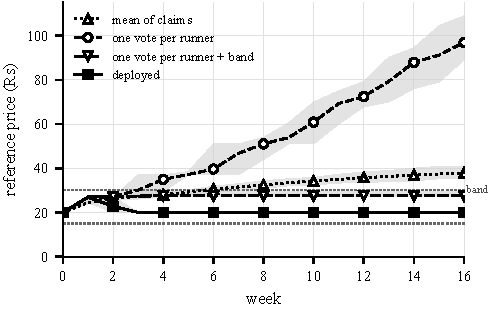
\includegraphics[width=\columnwidth]{figures/fig_reference.pdf}
\caption{Reference price week by week with 60\% of runners line-walking. Lines are
the mean over 30 seeds; shaded bands span the 5th to 95th percentile of seeds. The
deployed estimator rises while the near-line rule is still collecting four claims
from each attacker, then returns to the true price once their votes are excluded.}
\label{fig:reference}
\end{figure}

\emph{Why most evasive attackers were caught.} An evasive attacker inflates half of
their claims, so their long-run share of near-line claims is 0.50, and only 15--19\%
of them ever reached 60\% over their whole history. Yet 79--85\% were flagged. The
reason is in how the rule is evaluated, not in its threshold. It runs after every
claim, over the last 30 days, which for these runners holds about six judged claims.
With six fair coin flips, four or more heads has probability $22/64\approx0.34$, and
the rule gets a fresh chance at every submission. At the moment of flagging, the
window held on average 6.4 claims, of which 4.5 were near the line, a share of 0.72.
An attacker who wants to stay clear has to keep the \emph{windowed} share under 60\%,
which at this claim rate means inflating well under half the time.

\begin{table}[!t]
\caption{Money and Time to Detection Under the Deployed Estimator.
Mean (95\% CI Half-Width) Over 30 Seeds}
\label{tab:money}
\centering
\scriptsize
\setlength{\tabcolsep}{2.4pt}
\begin{tabular}{@{}lccccc@{}}
\toprule
& & Attackers & Days to & \multicolumn{2}{c}{Excess paid (Rs.)} \\
\cmidrule(l){5-6}
Strategy & Attackers & flagged & first flag & before flag & 16 weeks \\
\midrule
Line, 10\% & 4 & 100\% & 19.1 (2.0) & 110 (3) & 632 (20) \\
Line, 30\% & 12 & 100\% & 19.3 (1.2) & 331 (4) & 1958 (46) \\
Line, 60\% & 24 & 100\% & 19.0 (0.8) & 1016 (33) & 4370 (74) \\
Evasive, 10\% & 4 & 85\% & 48.0 (5.6) & 170 (12) & 316 (13) \\
Evasive, 30\% & 12 & 79\% & 46.4 (3.2) & 520 (21) & 954 (32) \\
Evasive, 60\% & 24 & 83\% & 45.3 (2.1) & 1019 (32) & 1986 (44) \\
Volume, 1 runner & 1 & 100\% & 3.8 (0.7) & 27 (1) & 1591 (46) \\
Overt, 60\% & 24 & n/a & n/a & $-167$ (8) & $-167$ (8) \\
\bottomrule
\multicolumn{6}{@{}p{0.97\columnwidth}@{}}{Excess paid is reimbursement above the
true price, summed over all attackers. ``Before flag'' counts claims made before each
attacker's first near-line flag; ``16 weeks'' assumes nobody reviews the flag.
Overt claims are flagged one by one and reimbursed at the reference, so overt
attackers recover less than they spend.}
\end{tabular}
\end{table}

\emph{Money and time.} Table~\ref{tab:money} reports what the attacks cost. The
near-line flag withholds nothing, by design, so the money only stops when an
administrator acts on it. Line-walkers were flagged after about 19 days, having
taken about Rs.~28 each by then. Evasive attackers who were flagged took about 46
days to reach it; counting the ones never flagged over their whole run, evasive
attackers took about Rs.~43 each outside any flag. The 16-week column is what the platform would pay if nobody
reviewed the flags. At 30\% line-walkers it is Rs.~1,958, about Rs.~7 per inflated
claim, which is why review capacity is part of the defence.

\emph{Names.} Binding a claim to the order's lines
(Section~\ref{sec:design-claims}) was tested with 61 names a runner might type for
three priced lines: misspellings, padded names (``chicken puff special''), obfuscated
ones (``ch1cken puff'', a Cyrillic letter, spaced letters), unrelated renames
(``snack'', ``zzq special''), and swaps to the name of an unpriced line on the same
order. Under the earlier rule, which matched names against the whole campus list, 41
of the 61 were paid unchecked. Under the deployed rule 20 are judged against the
right reference, 35 are refused, and none is judged against the wrong one. The six
that remain unchecked are the swaps. A runner can claim a priced item's money under
the name of a hand-typed, unpriced line on the same order, and that line has no
reference to judge it by. This is the cold-start case, and its bound is the escrow
hold: a payout above the hold freezes for review (Section~\ref{sec:eval-dispatch}).
The deterministic and fuzzy tiers also mapped 193 of 200 hand-written misspellings of
20 canteen items to the right key, none to a wrong one, and merged none of 20
look-alike items (``egg roll'', ``paneer tikka roll'') into a listed one. We wrote
all of these names ourselves, so the numbers measure coverage of the errors we
anticipated, not accuracy in the field.

\emph{Shops.} For shop-level pooling the same item was placed at a canteen charging
the reference and at dearer ones. Against the campus reference every honest claim at
a dearer counter is judged against Rs.~20, so an honest Rs.~30 claim is flagged and
Rs.~10 withheld for telling the truth. Table~\ref{tab:store}(a) shows when
\eqref{eq:store} has moved the shop's reference far enough. A shop charging Rs.~30
needs three distinct reporting runners and one charging Rs.~40 needs ten. A shop
charging Rs.~60 never gets there, because the drift cap holds its reference at
Rs.~50; such an item needs an administrator to list it separately. The same mechanism
is the weak point, and Table~\ref{tab:store}(b) measures it. The number of claims per
colluder made no difference at 1, 10 or 50, because each runner has one vote. The
number of colluders did. At a shop with few honest reporters, two or three colluders
claiming Rs.~30 were paid in full, Rs.~10 above the true price per claim; with ten or
twenty honest reporters they had to match them in number. Every colluding claim in
the Rs.~30 rows still counted toward the walking-the-line rule, which is judged
against the shop-adjusted reference, so colluders who keep doing it are flagged as
line-walkers after four claims. Seeding the shop is not free either: until three
distinct runners have reported there, each colluder's Rs.~30 claim is judged against
Rs.~20 and flagged, which counts toward the strike ladder.

\begin{table}[!t]
\caption{Shop-Level Pooling Against a Campus Reference of Rs.~20}
\label{tab:store}
\centering
\scriptsize
\setlength{\tabcolsep}{3pt}
\begin{tabular}{@{}cccc@{}}
\toprule
\multicolumn{4}{@{}l}{(a) Distinct honest reporters before an honest claim is paid in full} \\
Shop price & Reporters needed & Shop reference then & Withheld before \\
\midrule
Rs.~25 & 0 & 20.00 & 0 (within allowance) \\
Rs.~30 & 3 & 23.33 & Rs.~10 \\
Rs.~40 & 10 & 32.50 & Rs.~20 \\
Rs.~60 & never (cap Rs.~50) & 50.00 & Rs.~10 at 20 reporters \\
\midrule
\multicolumn{4}{@{}l}{(b) Colluders needed to be paid in full at a Rs.~20 shop} \\
Honest reporters & Claiming Rs.~30 & Claiming Rs.~40 & Claiming Rs.~50 \\
\midrule
0 & 3 & 10 & 20 \\
1 & 2 & 8 & 20 \\
3 & 3 & 8 & 15 \\
5 & 5 & 8 & 15 \\
10 & 10 & 11 & 11 \\
20 & 20 & $>$20 & $>$20 \\
\bottomrule
\multicolumn{4}{@{}p{0.95\columnwidth}@{}}{Every colluder files 1, 10 or 50 claims;
the counts are identical in all three cases. Honest reporters each claim Rs.~20
twice.}
\end{tabular}
\end{table}


\subsection{Reputation Farming}\label{sec:eval-farming}
% Experiment 5: backend/evals/paper/exp5_farming.py
We built rating histories for several attackers and passed them through the
production profile builder and farming detectors. The benchmark is an honest runner
rated five stars by twenty strangers, whose ranking score is 4.57. An honest runner
rated by twenty strangers (mostly five stars) and five friends scores 4.52, so a
normal share of friends among one's customers costs nothing.

Fig.~\ref{fig:farming}(a) follows a runner who served six strangers badly (mean 3.0),
was penalised, and then collected five-star ratings from three friends. The plain
average climbs to 4.96. Weighting each rating, which is how the system worked before
it moved to one vote per rater, lets the farmed score pass the honest benchmark at
160 ratings. The deployed weighting stays between 3.21 and 3.65 however many ratings
are farmed, because three friends remain three votes and their weight falls as their
share of the history grows. With eight friends the deployed score peaks at 3.83. On
the ranking scale of~\eqref{eq:effective}, this is the difference between the honest
runner's 857~m advantage and at most 263~m for the farmer. The farming detectors
flagged every history with 20 or more farmed ratings, whether the runner had been
penalised or was farming from a standing start.

The breadth attack (Fig.~\ref{fig:farming}(b)) is the limit. If every farmed rating
comes from a different
friend, one rating each, one vote per rater gives no protection: eighty such friends
reproduce the honest benchmark of 4.57 exactly, and none of the three detectors fires
because no friend rates twice and there is no stranger to compare against. The attack
needs eighty real, verified accounts that have accepted a friend request and each paid
for a real errand, and friendship maturity (Section~\ref{sec:design-trust}) makes the
new ties count for less in trust, though not in reputation. We do not defend against
it beyond that cost.

\begin{figure}[!t]
\centering
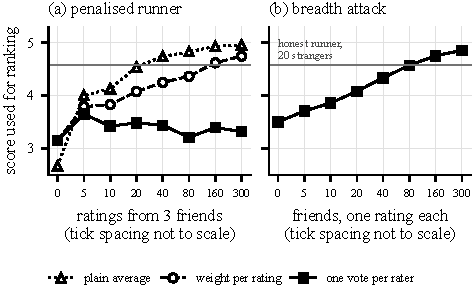
\includegraphics[width=\columnwidth]{figures/fig_farming.pdf}
\caption{(a) Ranking score of a penalised runner as three friends add five-star
ratings, under three weightings. (b) The breadth attack under the deployed weighting,
in which each rating comes from a different friend. The horizontal axes are
categorical and roughly doubling, not linear. The histories are constructed, not
sampled, so there is no seed variation to show.}
\label{fig:farming}
\end{figure}


\subsection{Dispatch and Escrow}\label{sec:eval-dispatch}
% Experiment 6: backend/evals/paper/exp6_dispatch.py   (30 seeds)
% Experiment 7: backend/evals/paper/exp7_escrow.py     (30 seeds; frontier 10)
Table~\ref{tab:dispatch} dispatches the same 30 simulated semesters (routine regime,
about 26,000 errands each) in four ways. Each runner's willingness and response delay
for a given errand are fixed by a seed shared across policies, so the policies differ
only in when each runner is told.

\emph{Ranking alone does little.} Ranking a simultaneous broadcast by trust left
17.8\% of errands with a runner within two hops. When every candidate is told at
once, the order of the list cannot change who answers first. Staging the same offers
in time doubled that to 35.8\%, at a cost of 6.7~s in median wait and 42~s at the
90th percentile. Offering to one runner at a time in trust order reached 50.4\% but
more than doubled the median wait again.

\emph{The router creates in-group circulation.} The same table measures the effect
that motivates Section~\ref{sec:design-policy}. Staging doubled the share of an
honest group's errands that stayed inside the group, from 3.5\% to 7.0\%, and
one-at-a-time dispatch raised it to 12.1\%. No group member chose this; the router
did. This is the circulation the ring detector reads, and it is why the detector
must be conditioned on the router.

\emph{The control group is not free.} The 5\% coin is tossed for each logged first
offer, and an errand whose friends-first round finds nobody is tossed again for the
unrestricted round, so 7.0\% of errands went out exploratory. Of those, 12.8\% went
to a runner within two hops, against 37.5\% in regular rounds.

\emph{The scheduler fix.} When a requester has no friend or friend-of-friend among the
five nearest runners, the first offer goes straight to those five. Under the original
scheduler such an errand was never widened, and 4.4\% of them went unaccepted for 30
minutes, which made staged dispatch the only policy with an overall expiry rate of
1.9\%. With the 90-second widening applied to these errands too, their expiry fell
to 0.23\%, the same as the other policies, while the share taken within two hops
moved only from 36.2\% to 35.8\%.

\begin{table}[!t]
\caption{Dispatch Policies on the Same Simulated Semesters.
Mean (95\% CI Half-Width) Over 30 Seeds}
\label{tab:dispatch}
\centering
\scriptsize
\setlength{\tabcolsep}{1.6pt}
\begin{tabular}{@{}lcccc@{}}
\toprule
& Broadcast, & \multicolumn{2}{c}{Staged} & One at \\
\cmidrule(lr){3-4}
& ranked & fixed & original & a time \\
\midrule
Taken within 2 hops (\%) & 17.8 (0.1) & 35.8 (0.2) & 36.2 (0.2) & 50.4 (0.3) \\
By a direct friend (\%) & 5.1 (0.1) & 10.3 (0.1) & 10.4 (0.1) & 18.0 (0.1) \\
Honest group's errands kept inside (\%) & 3.5 (0.1) & 7.0 (0.2) & 7.0 (0.2) & 12.1 (0.3) \\
Median wait (s) & 12.3 (0.0) & 19.0 (0.1) & 18.6 (0.1) & 41.9 (0.1) \\
90th-percentile wait (s) & 36.7 (0.2) & 78.9 (0.1) & 76.8 (0.1) & 122.2 (0.4) \\
Unaccepted after 30 min (\%) & 0.22 (0.01) & 0.22 (0.01) & 1.88 (0.03) & 0.22 (0.01) \\
\quad unrestricted first offer (\%) & n/a & 0.23 (0.02) & 4.38 (0.06) & n/a \\
\bottomrule
\multicolumn{5}{@{}p{0.97\columnwidth}@{}}{``Original'' is the scheduler before the
fix in Section~\ref{sec:impl}. About 40\% of staged errands had no friend or
friend-of-friend among the five nearest runners and went out unrestricted.}
\end{tabular}
\end{table}

\emph{Escrow.} We drew 3,000 orders per seed, mixing MRP goods with one to four
loose-priced lines, and assumed that a loose item costs its listed price 70\% of the
time and 10\%, 20\% or 35\% more otherwise. Each line was judged by the production
judge and each hold computed by the production ledger code. With no headroom,
56\% of payouts would freeze for review. Fig.~\ref{fig:escrow} traces the trade-off
as the headroom grows. For about the same money locked without need (Rs.~17--18 per
order), headroom on loose-priced items alone froze 3.5\% of payouts against 7.0\% for
headroom on the whole order, and full protection needed Rs.~39 against Rs.~87. The
deployed 16\% froze 9.0\% (95\% CI $\pm0.2$) of payouts while locking Rs.~12.7 per
order. Under a dearer price model, in which half of all loose items cost 10--60\%
more than listed, it froze 18.4\%, and the advantage of targeting the uncertain part
held along the whole curve. The same headroom bounds the cold-start case of
Section~\ref{sec:design-reference}: an unpriced line can be over-claimed only up to
the slack in the hold, Rs.~12.7 per order on average and Rs.~32 at the 95th
percentile here, before the payout freezes for a person to look at.

\begin{figure}[!t]
\centering
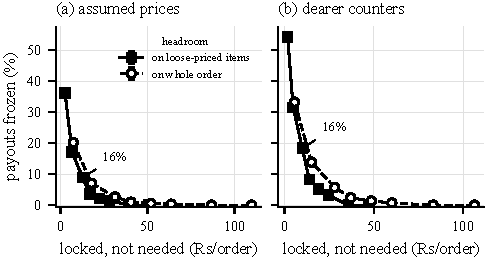
\includegraphics[width=\columnwidth]{figures/fig_escrow.pdf}
\caption{Payouts frozen for review against money locked without need, as escrow
headroom rises from 5\% to 50\%, for two choices of what the headroom covers, under
(a) the assumed price model and (b) a dearer one. Error bars are 95\% confidence
intervals over 10 seeds of 3,000 orders.}
\label{fig:escrow}
\end{figure}


\subsection{System Measurements}\label{sec:eval-system}
% Experiment 8: backend/evals/paper/exp8_scale.py   (run alone; five repetitions)
% Language channels: backend/evals/run_eval.py --repeats 5
\emph{Cost.} Table~\ref{tab:scale} times the evidence pipeline on synthetic campuses
of 1,200 to 10,000 students with about 20 payments each, against one Neo4j 5.26
instance. Each graph job was run five times on the loaded graph and we report the
median with the range; each trust lookup is one call of the production
\code{social\_scores} for five candidates, timed over 50 calls after 10 discarded
warm-up calls. The experiment ran alone on the machine described in
Section~\ref{sec:eval-method}. At 10,000 students the three graph jobs together took
11.9~s, against a scheduler that runs them every ten minutes, and the trust lookup on
the dispatch path took 3.0~ms at the median and 4.2~ms at the 95th percentile. The
ring search now returns every ring, 117 of them on the largest synthetic campus,
whose random payments close many cycles; this is what the earlier cap of 50 hid. The
production Tarjan routine processed a million nodes and three million edges in
9.4~s, and fitting the acceptance model took 2.5~s on 10,000 logged rounds and 25~s
on 100,000, about a semester's rounds for a campus of 5,000 students.

\begin{table*}[!t]
\caption{Cost of the Evidence Pipeline. Median (Range) of Five Repetitions}
\label{tab:scale}
\centering
\footnotesize
\setlength{\tabcolsep}{6pt}
\begin{tabular}{@{}rrrcccc@{}}
\toprule
& & & \multicolumn{3}{c}{Graph jobs (s)} & Trust lookup \\
\cmidrule(lr){4-6}
Students & Friendships & Payments & Closure & Circulation & Rings & p50 / p95 (ms) \\
\midrule
1,200 & 4,050 & 23,944 & 0.11 (0.06--0.14) & 0.81 (0.63--0.93) & 0.51 (0.50--0.54) & 5.7 / 14.8 \\
2,500 & 8,408 & 49,895 & 0.14 (0.12--1.16) & 1.65 (1.57--2.90) & 1.25 (1.05--1.41) & 10.9 / 16.5 \\
5,000 & 16,862 & 99,787 & 0.32 (0.26--0.40) & 3.19 (3.04--3.91) & 2.41 (2.20--2.63) & 4.0 / 6.3 \\
10,000 & 33,755 & 199,525 & 0.54 (0.49--0.88) & 6.53 (6.13--7.27) & 4.91 (4.59--4.95) & 3.0 / 4.2 \\
\midrule
\multicolumn{7}{@{}l}{Tarjan routine alone, 3 out-edges per node: $10^4$ nodes 0.03~s;
$10^5$ nodes 0.66~s; $10^6$ nodes 9.4~s} \\
\multicolumn{7}{@{}l}{Acceptance-model fit: $10^3$ rounds 0.24~s; $10^4$ rounds 2.5~s;
$10^5$ rounds 25~s} \\
\bottomrule
\multicolumn{7}{@{}p{0.8\textwidth}@{}}{\scriptsize Hardware: Intel Core i7-12650H, 16 threads,
7.6~GiB available to Docker; Python 3.12; Neo4j 5.26 Community. Trust lookups: 50
timed calls after 10 warm-up calls, five candidates each.}
\end{tabular}
\end{table*}

\emph{Language channels.} The advisory channels play a small part in this design,
and we tested them only for that part. On eleven hand-written cases with five runs
each, the errand-text channel scored genuine groups 41.7 points higher than farmed
ones on a 0--100 scale and cleared every honest control, but it also cleared one of
three farmed groups whose errands had been written to look varied. The
rating-comment channel showed no separation ($-1.2$ points) and failed to clear an
honest runner whose friends rate without comments, so it is switched off. Neither
channel followed instructions injected into the text. The cases were written by the
authors, and the harness refuses to report an accuracy figure until twenty
blind-labelled pilot cases exist, so these numbers show only that the errand-text
channel works end to end, not that it is accurate.

\emph{Tests.} The full suite of 273 automated tests, including at least one
regression test for each of the six faults in Section~\ref{sec:impl}, passed in
111~s.


%======================================================================
\section{Discussion and Limitations}\label{sec:discussion}
%======================================================================
\subsection{What Relational Evidence Cannot Separate}
A group of friends that deliberately routes favours to each other and a ring that
farms ratings produce the same structure, the same money cycles and the same
deliberate routing. Nothing in the friendship graph, the payment graph or the offer
log distinguishes them; only intent does. This is an identifiability limit, not a
tuning problem. The policy test asks whether a group took its own errands more often
than friends elsewhere on campus do. Honest favour-trading answers yes for the same
reason a ring does, and a careful ring that farms only as often as ordinary friends
help each other answers no. Fig.~\ref{fig:sweeps} shows both ends: honest groups are
flagged once favours become frequent, and the deployed test loses coordinated rings
as they farm less. Only the content of the errands or a person can separate the two
cases, and our language channel is not yet reliable enough to lean on
(Section~\ref{sec:eval-system}). We therefore keep a person between every ring flag
and any sanction: ring and farming flags never feed the automatic ladder, and the
automated parts of the system may demote and pause but never exclude.

\subsection{Why the First Policy Test Failed}
The first version of the test used the router's own logged scores as its model of
who would accept an errand. Within a tier every candidate is notified at once, so the
order of the list has little effect on who answers first, and the scores overstated
how much the router decides. A coordinated ring exploited exactly that. When the
partner is always the router's first choice, a test that believes the router expects
the partner to take the errand nearly every time and finds nothing surprising. Three
results in Section~\ref{sec:eval-policy} point to the same cause. Exploration helped
only slowly, setting the trust weight in the expectation to zero restored recall, and
an acceptance model fitted to what runners actually did restored most of it at the
deployed exploration rate, without that cost. The general lesson is that a detector
conditioned on a matcher should condition on the matcher's measured effect, not on
its design weights.

\subsection{Limitations}
Every result here is from simulation. The friendship graph is a block model, not a
real campus, and runner behaviour (willingness, response delay, friend affinity) is
assumed. We varied the parameters that matter most, and the confidence intervals
describe variation across seeds of that model, not uncertainty about whether the
model is right. A pilot may find behaviour we did not imagine. The thresholds in
Table~\ref{tab:params} are reasoned defaults, not values fitted to data; the offer log
exists partly so that a pilot can fit them. The acceptance model has four features,
and a ring that varies distance and timing to look like an ordinary friend will be
harder to separate than the coordinated rings simulated here. A ring whose members
never declare friendship is invisible to every friendship-based mechanism, at the
price of forgoing the trust boost; its cycles would appear only in the any-pair cycle
search, which flags too many honest students to act on. The breadth attack defeats the
reputation weighting at the cost of eighty real accounts. At a shop with few honest
reporters, two or three colluders can move its reference, although the near-line rule
still sees them. A runner can still claim a priced item's money under the name of an
unpriced line on the same order, bounded only by the escrow hold. Line-walkers keep
being paid the allowance until an administrator reviews the flag, so review capacity
is part of the defence. Finally, the language-channel evaluation uses eleven
hand-written cases.

\subsection{Ethics and Deployment}
These mechanisms withhold money and can pause or suspend students, so we built them
around three rules. Automated components may warn, demote and pause, but only a person
may exclude: account suspension needs flags an administrator has upheld. Every flag
carries the evidence that raised it, every sanction tells the student why, and a
dismissed flag releases the money and lifts the pause it caused. And the advisory
model runs on campus hardware, so that students' errand notes and reviews do not
leave the institution. A pilot will collect data about identifiable students and will
need institutional ethics approval and informed consent before it begins.

\subsection{Beyond Campus Errands}
Nothing in the design is specific to food. It applies wherever expenses are reported
rather than documented, such as shared purchasing in hostels or offices and informal
neighbourhood delivery, and more generally to any platform that uses social ties both
to route work and to look for collusion. Once the router shapes who meets whom, the
fraud detector must account for the router, or it ends up auditing the router's
choices instead of people's.


%======================================================================
\section{Conclusion}\label{sec:conclusion}
%======================================================================
Remove the receipt from a delivery platform and every fraud control has to infer
instead of verify. We built Errandly's controls around that fact. Price claims are
bound to the lines the requester ordered and judged against a reference learned with
one vote per runner inside a human-set band, and runners who habitually claim just
under the limit lose their vote. Social closure discounts trust but never accuses; an
accusation needs money cycling among mutual friends. And because the dispatcher's own
preference for friends creates in-group circulation, ring flags are tested against an
acceptance model fitted to how students outside every suspected group actually
respond to offers.

In simulation the cycle search found rings that structure-only, money-only and
graph-mining baselines missed, and the policy test removed most of the false flags
that the router's preference for friends had caused. The test's first version failed
in a way we did not anticipate: by borrowing the router's own weights as its model of
behaviour, it cleared almost every coordinated ring. Fitting that model to logged
acceptances repaired most of the failure without the service cost of more
exploration. What no version can repair is the case in which honest friends and a
careful ring route errands to each other in the same way; there, only a person who
reads the errands can decide. The next step is a pilot with ethics approval, which
can replace our assumed behaviour and hand-set thresholds with measured ones.


\section*{Author Contributions}
C.~M.~Mattam designed and built the backend services, the event pipeline, the
mobile client and the social trust graph. U.~Gogoi designed and built the escrow and
payment flow and the price-claim fraud controls, and ran the evaluation.
S.~Sajlal built the web and administrator client, tested the applications, and
contributed the literature review and the editing of the manuscript. R.~S supervised
the work and reviewed the manuscript. All authors approved the final version.

\section*{Data and Code Availability}
The source code, the experiment scripts and the result files with their
seeds are in the project repository at the commit named in each result file. The
README in \code{backend/evals/paper} gives the command that regenerates every table
and figure. No data about real students were collected.

\section*{Acknowledgment}
The authors thank the School of Computer Science and Engineering, Vellore Institute
of Technology, for supporting this work. The authors used an AI writing and coding
assistant (Claude, Anthropic) to help draft and edit the text of this manuscript and
to write the evaluation scripts; the authors reviewed and verified all content,
code and results and take full responsibility for them.

\bibliographystyle{IEEEtran}
\bibliography{refs}

% Biographies are required by IEEE Access at submission. Each author should
% rewrite their own; IEEE Access also asks for a photo with the final files
% (replace IEEEbiographynophoto with IEEEbiography and a photo then).
\begin{IEEEbiographynophoto}{Chris Martin Mattam}
is working toward the B.Tech. degree in computer science and engineering at Vellore
Institute of Technology (VIT), Vellore, India.
\end{IEEEbiographynophoto}

\begin{IEEEbiographynophoto}{Ujjwal Gogoi}
is working toward the B.Tech. degree in computer science and engineering at Vellore
Institute of Technology (VIT), Vellore, India.
\end{IEEEbiographynophoto}

\begin{IEEEbiographynophoto}{Sanskriti Sajlal}
is working toward the B.Tech. degree in computer science and engineering at Vellore
Institute of Technology (VIT), Vellore, India.
\end{IEEEbiographynophoto}

\begin{IEEEbiographynophoto}{Ranjithkumar S}
is an Assistant Professor with the School of Computer Science and Engineering, Vellore
Institute of Technology (VIT), Vellore, India.
\end{IEEEbiographynophoto}

\vfill

\end{document}
